% !TEX program = xelatex
\documentclass[UTF8,a4paper,zihao=-4,fontset=windows]{ctexart}
\usepackage[margin=3cm]{geometry}
\usepackage{amsmath,amssymb,booktabs,array,tabularx,longtable,graphicx}
\usepackage{enumitem,caption,float,placeins,xcolor,fancyhdr,fvextra,needspace}
\usepackage{xurl}
\usepackage[hidelinks,unicode]{hyperref}
\usepackage{microtype}
\setmonofont{Consolas}
\xeCJKDeclareCharClass{CJK}{"2103}
\setlength{\parindent}{2em}
\setlength{\parskip}{0.12em}
\setlength{\emergencystretch}{3em}
\linespread{1.12}
\setlist{nosep,leftmargin=2em}
\captionsetup{font=small,labelfont=bf,labelsep=quad,skip=5pt}
\ctexset{section={format=\centering\Large\bfseries,beforeskip=1.1ex plus .4ex,afterskip=.65ex},subsection={format=\large\bfseries,beforeskip=.85ex plus .3ex,afterskip=.5ex},subsubsection={format=\normalsize\bfseries}}
\pagestyle{fancy}
\fancyhf{}
\fancyfoot[C]{\thepage}
\renewcommand{\headrulewidth}{0pt}
\setlength{\headheight}{14pt}
\setlength{\footskip}{18pt}
\renewcommand{\arraystretch}{1.18}
\renewcommand{\topfraction}{0.95}
\renewcommand{\bottomfraction}{0.9}
\renewcommand{\textfraction}{0.05}
\renewcommand{\floatpagefraction}{0.8}
\setcounter{topnumber}{4}
\setcounter{totalnumber}{5}
\setlength{\textfloatsep}{11pt plus 2pt minus 2pt}
\setlength{\floatsep}{9pt plus 2pt minus 2pt}
\newcommand{\unit}[1]{\ensuremath{\,\mathrm{#1}}}
\newcommand{\celsius}{\ensuremath{\,{}^\circ\mathrm{C}}}
\newcommand{\Cmax}{C_{\max}}
\newcommand{\rhoe}{\rho_{\mathrm{eff}}}
\newcommand{\rhod}{\rho_{\mathrm d}}
\newcommand{\Ds}{\mathrm D_{\mathrm s}}
\newcommand{\dd}{\mathop{}\!\mathrm d}
\newcommand{\sourcecode}[2]{\Needspace{6\baselineskip}\subsection{#1}\noindent{\footnotesize\nolinkurl{#2}}\par\smallskip\VerbatimInput[fontsize=\fontsize{8}{9.5}\selectfont,breaklines=true,breakanywhere=true,numbers=left,numbersep=4pt,xleftmargin=1.6em,frame=single,framesep=3pt]{#2}\par}
\newcommand{\codegroup}[1]{\Needspace{10\baselineskip}\subsection{#1}}
\hypersetup{pdftitle={考虑变物性与径向收缩的圆柱药材干燥模型},pdfauthor={},pdfsubject={四问论文初稿},pdfkeywords={药材干燥,变物性,热质耦合,有限体积,严格阈值}}
\begin{document}
\begin{center}
{\LARGE\bfseries 考虑变物性与径向收缩的圆柱药材干燥模型\par}
\vspace{0.7em}
{\large\bfseries 摘\quad 要}
\end{center}
\begingroup
\linespread{1}\fontsize{11.5}{18}\selectfont
\setlength{\parindent}{2em}
\setlength{\parskip}{5pt}
\noindent\hspace*{2em}针对圆柱药材热风干燥过程中的内部温湿分布预测与干燥时间判定问题，本文依据题给环境记录、材料物性及观测半径，构建由常热物性到变物性、由固定几何到径向收缩的递进式传热传质模型。在有效湿度边界、不显式计入潜热及所设后段环境条件下，预测规定时刻与位置的温度和干基含水率，并确定达到规定含水率阈值所需的模型干燥时长。

\textbf{针对问题一}，将药材近似为轴对称圆柱体，采用常热物性并考虑水分扩散系数随含水率变化，建立一维径向温湿传递模型。利用\textbf{圆环有限体积法}共享相邻单元面通量，并采用\textbf{隐式BDF方法}积分，求得预热阶段的径向温湿分布。计算得到1800\unit{s}时轴心与表面温度分别为\textbf{33.5753\celsius}和\textbf{36.7856\celsius}，表面含水率降至\textbf{1.5102\unit{kg/kg}}，轴心仍接近初始值\textbf{2.55\unit{kg/kg}}。\textbf{结果表明，热量已传入内部而失水仍集中于外层，传热与水分扩散具有不同的时间尺度。}

\textbf{针对问题二}，进一步考虑热容量、导热率和扩散率随局部状态变化的反馈，从共同初态建立\textbf{变物性热质耦合模型}。采用Chebyshev配点与Radau隐式积分联立求解全过程温湿场，并通过\textbf{扩散系数的对数分解}区分升温促进与失水抑制作用。计算得到3\unit{h}时轴心与表面温差仅0.1169\unit{K}，含水率差仍为\textbf{0.7581\unit{kg/kg}}；2.5--3\unit{h}内两处扩散率均已回落。\textbf{结果表明，温度场趋于均匀时，含水率仍存在明显的径向梯度。}

\textbf{针对问题三}，在第二问一维径向有效模型的基础上，以全径向最大含水率严格低于0.15\unit{kg/kg}为停止条件，建立干燥终点判定模型。采用\textbf{重构极值搜索}追踪径向含水率的最大值，计算发现临近干燥终点时轴心含水率仍为径向最大值，因此以轴心达标确定干燥终点。结合网格加密和独立时间积分检验设置数值裕量，在4\unit{h}后环境保持末小时均值的假设下，得到\textbf{达到规定含水率要求所需的模型干燥时长为57.4741\unit{h}。}

\textbf{针对问题四}，根据附件2的观测半径，在恒长度、均匀径向收缩假设下，由\textbf{干物质守恒}构建\textbf{材料坐标模型}，将移动边界转化为固定参考域，避免重复加入干基含水率的体积浓缩项。采用该问物性从初态求解，在同一后段环境假设下得到一维径向模型的执行时长\textbf{51.0921\unit{h}}。进一步设置\textbf{同物性恒半径对照}，其临界时间为129.8484\unit{h}；\textbf{施加观测收缩后，模型临界时间缩短约60.65\%。}

\vspace{0.7em}
\noindent\textbf{关键词：}药材干燥；变物性；热质耦合；径向收缩；阈值事件
\par\endgroup
\clearpage
\label{body:start}
\begingroup
\linespread{1.30}\selectfont
\setlength{\parskip}{5pt plus 1pt minus 1pt}
\setlength{\abovedisplayskip}{12pt plus 2pt minus 2pt}
\setlength{\belowdisplayskip}{12pt plus 2pt minus 2pt}
\setlength{\abovedisplayshortskip}{8pt plus 2pt minus 1pt}
\setlength{\belowdisplayshortskip}{10pt plus 2pt minus 2pt}
\ctexset{section={beforeskip=13pt plus 2pt minus 2pt,afterskip=7pt plus 1pt minus 1pt},subsection={beforeskip=10pt plus 2pt minus 1pt,afterskip=5pt plus 1pt minus 1pt},subsubsection={beforeskip=8pt,afterskip=4pt}}
\ctexset{section={number=\chinese{section},aftername=、,runin=false}}
\setlist{topsep=6pt,itemsep=3pt,parsep=0pt,partopsep=0pt,leftmargin=2em}
\renewcommand{\arraystretch}{1.30}
\captionsetup{skip=8pt}
\setlength{\textfloatsep}{16pt plus 2pt minus 2pt}
\setlength{\intextsep}{16pt plus 2pt minus 2pt}
\setlength{\floatsep}{14pt plus 2pt minus 2pt}
\clubpenalty=10000
\widowpenalty=10000
\displaywidowpenalty=10000
\raggedbottom
\renewcommand{\thetable}{S\arabic{table}}
\renewcommand{\theHtable}{pre.\arabic{table}}
\section{问题重述}
\subsection{问题背景}
干燥是影响中药材成品品质的重要工序，热风烘干通常包括预热平衡与恒温干燥两个阶段。烘房环境通过表面换热和水分交换改变药材内部状态，热量向内传递、水分向外迁移，并可能伴随尺寸收缩。由于内部传输需要时间，表面的升温或失水不能直接代表内部各处的状态。因此，需要建立温度与含水率随时间、位置变化的模型，在给出内部状态预测的同时，确定满足干燥要求所需的时间。

题设药材近似为长25\unit{cm}、初始半径2\unit{cm}的圆柱，初始温度为28\celsius，干基含水率为2.55\unit{kg/kg}。已知资料包括烘房温湿环境记录、药材半径记录和各问的物性参数。

\subsection{问题提出}
根据上述条件，建立模型完成以下四项任务。论文表格与完整过程文件分别按题设要求输出，结果统一保留四位小数。

\textbf{问题一：}采用附录2参数，建立1800\unit{s}预热阶段的温度与含水率模型。在论文中给出100、300、600、900、1200、1500、1800\unit{s}及到中心距离0、0.5、1、1.5、2\unit{cm}处的温湿结果；完整结果按1\unit{s}和0.1\unit{cm}采样，写入\texttt{result1.xlsx}。

\textbf{问题二：}全程统一采用附录3经验公式，描述整个烘干过程的温度与含水率变化。在论文中给出前3\unit{h}每隔0.5\unit{h}、上述五个位置的温湿结果；完整过程按1\unit{s}和0.1\unit{cm}采样，写入\texttt{result2.xlsx}。

\textbf{问题三：}依据药材各处含水率低于0.15\unit{kg/kg}的要求，确定以小时计的烘干时长。论文表格列出每隔6\unit{h}及结束时刻、每隔0.5\unit{cm}的含水率；完整过程按60\unit{s}和0.1\unit{cm}采样，写入\texttt{result3.xlsx}。

\textbf{问题四：}结合附件2半径记录与附录4物性，确定尺寸收缩下的烘干时长。论文表格列出每隔6\unit{h}及结束时刻、实际材料范围内每隔0.5\unit{cm}和当前表面的含水率；完整过程按60\unit{s}和0.1\unit{cm}采样，写入\texttt{result4.xlsx}。

\section{问题分析}
\textbf{对于问题一，}重点是描述预热阶段内部与表面响应的空间差异。附录2的热物性为常数，水分扩散系数随含水率变化，因而可分别建立导热方程与非线性扩散方程，以初始均匀状态、轴心对称条件和表面交换条件构成定解问题。采用圆环有限体积法共享相邻单元面通量，并通过隐式积分获得规定点值与完整过程\cite{dasilva2014}。

\textbf{对于问题二，}物性随局部温度或含水率改变，温度与水分场之间形成反馈，需从共同初态联立求解变物性方程。前3\unit{h}规定表应从同一全过程轨迹提取，不接续第一问末态。采用Chebyshev配点与隐式积分处理空间梯度和长时演化，同时分析升温与失水对扩散系数的共同作用；观测时段之后的环境按明确的延拓假设处理。

\textbf{对于问题三，}难点在于把“各处低于阈值”转化为可计算的终止条件。沿用第二问轨迹，追踪全径向最大含水率，并检查重构曲线的内部极值，避免只凭表面值或平均值判断结束。先定位最大值等于阈值的事件根，再结合加密与独立积分检验设置数值余量，选取严格低于阈值的执行点；判定使用未舍入值，表格仅承担结果展示。

\textbf{对于问题四，}半径变化使计算区域和表面位置随时间移动，固定网格上的距离不再直接对应同一材料位置。以干物质守恒为基础建立材料坐标方程，将变动区域映射到固定参考域，并按附录4物性从共同初态独立积分。恒长度、均匀径向收缩是对内部运动的附加假设\cite{adrover2020,wu2022}，其他物料的经验参数不直接迁移。输出时区分实际域内位置与当前表面，并以同物性恒半径条件对照分析收缩的作用。

主模型的空间近似见假设\ref{ass:midsection}。有限圆柱全域终点还需结合相应二维证据判断，不能由一维阈值事件直接推出；统一适用边界见第\ref{sec:limitations}节。

\section{模型假设}
\label{sec:assumptions}
\begin{enumerate}
\item 假设药材为轴对称连续介质，初始温度、干基含水率及干密度在空间上均匀分布。\label{ass:midsection}
主模型采用中截面径向近似，忽略端面影响。
\item 假设烘房环境在空间上均匀，题给空气水分量可等效作为药材表面传质的有效环境边界量。
\item 假设药材表面的传热、传质通量分别与温度差和有效含水率差成正比，各问沿用同一组恒定交换系数。
\item 假设烘干过程中药材干物质质量守恒，题给密度仅用于有效热容量。
模型不显式计入水分蒸发潜热、水分迁移携焓及机械功。
\item 前三问假设药材尺寸保持不变；第四问假设药材长度不变，并随观测半径作均匀径向收缩。
\item 假设4\unit{h}后烘房环境保持稳定，其温度和空气水分量取3--4\unit{h}观测数据的算术平均值。
按末小时61个采样点计算，相应环境平台为
\begin{equation}
T_a=49.9989344262\celsius,\qquad b=0.04998754098\unit{kg/kg}.
\label{eq:future}
\end{equation}
\end{enumerate}

\Needspace{22\baselineskip}
\section{符号说明}
\begin{table}[H]
\centering\small
\caption{主要符号及单位}\label{tab:symbols}
\renewcommand{\arraystretch}{1.10}
\begin{tabularx}{\linewidth}{@{}lXl@{}}
\toprule 符号&含义&单位\\\midrule
$T$&材料摄氏温度&$^\circ\mathrm C$\\
$T_K$&材料绝对温度，$T_K=T+273.15$&$\mathrm K$\\
$C$&材料干基含水率，$C=m_w/m_d$&$\mathrm{kg/kg}$\\
$b$&有效材料边界值&$\mathrm{kg/kg}$\\
$r$&径向坐标&$\mathrm m$\\
$z$&轴向坐标&$\mathrm m$\\
$R$&当前外半径&$\mathrm m$\\
$L$&药材总长度&$\mathrm m$\\
$\rhoe$&有效热容量采用的经验密度&$\mathrm{kg/m^3}$\\
$\rhod$&单位当前体积的干物质密度&$\mathrm{kg/m^3}$\\
$c_p$&比热容&$\mathrm{J/(kg\cdot K)}$\\
$k$&导热系数&$\mathrm{W/(m\cdot K)}$\\
$D$&有效水分扩散系数&$\mathrm{m^2/s}$\\
$v_s$&材料速度&$\mathrm{m/s}$\\
$J$&材料映射的体积雅可比&$1$\\
$\xi$&参考坐标，$\xi=r/R$&$1$\\
$x$&配点坐标，$x=\xi^2$&$1$\\
$t_*$&最大含水率等于阈值的临界时刻&$\mathrm s$\\
$t_{\mathrm{exec}}$&正式执行时刻&$\mathrm s$\\
\bottomrule
\end{tabularx}
\end{table}

\Needspace{7\baselineskip}
\section{统一传热传质模型与数值方法}
\label{sec:common-model}
本节给出四问共用的局部收支关系。第一问在固定圆柱内代入常热物性并作
圆环积分，第二问将局部变物性代入并联立求解；第三问在第二问轨迹上求
严格阈值的执行时刻，第四问再通过材料坐标处理观测收缩。相应的方程化简
与求解步骤分别见第\ref{sec:q1}--\ref{sec:q4}节。
依假设\ref{ass:midsection}，主模型的温度、含水率及局部物性仅随径向位置和时间变化；题表的“到药材中心距离”按轴向中截面内的径向位置解释。
\Needspace{8\baselineskip}
\subsection{通用方程与初边值条件}
设$\Ds/\dd t=\partial_t+v_s\cdot\nabla$为材料导数。以
$\boldsymbol j_T=-k(C)\nabla T$表示导热通量，并用题给有效容量
$\rhoe c_p$描述局部温升率；将单位体积的有效热储存率等同于导热净输入
$-\nabla\cdot\boldsymbol j_T$，得到
\begin{equation}
\rhoe(C)c_p(C)\frac{\Ds T}{\dd t}
=\nabla\cdot\bigl(k(C)\nabla T\bigr).
\label{eq:heat}
\end{equation}
式\eqref{eq:heat}采用上述有效容量闭合，没有蒸发潜热或组分携焓项，
不是对真实总焓守恒的证明。对随干骨架运动的控制体$V_s(t)$，干物质不穿过
边界；内部不考虑压力驱动流动及流体相对干骨架的对流，水分仅以相对材料的扩散通量$\boldsymbol j_w=-\rhod D\nabla C$交换。
记外法向为$n$，则
\begin{equation}
\begin{aligned}
\frac{\dd}{\dd t}\int_{V_s(t)}\rhod\,\dd V&=0,\\
\frac{\dd}{\dd t}\int_{V_s(t)}\rhod C\,\dd V
&=-\int_{\partial V_s(t)}\boldsymbol j_w\cdot n\,\dd A.
\end{aligned}
\label{eq:material-balances}
\end{equation}
将式\eqref{eq:material-balances}用输运定理展开，再从水分方程中减去
$C$倍的干物质方程，得到
\begin{equation}
\partial_t\rhod+\nabla\cdot(\rhod v_s)=0,\qquad
\rhod\frac{\Ds C}{\dd t}=\nabla\cdot\bigl(\rhod D(T,C)\nabla C\bigr).
\label{eq:moisture}
\end{equation}
由初始干密度均匀以及固定骨架或均匀径向收缩的假设，$\rhod$保持空间均匀，可以从水分方程约去；时间变化的体积不应再向干基变量额外添加浓缩源。将内部外向通量与表面对流交换相等，水分条件按同一干质量标度约去$\rhod$，得到
\begin{equation}
-k\partial_nT=h_T(T_s-T_a),\qquad
-D\partial_nC=h_m(C_s-b).
\label{eq:boundary}
\end{equation}
当$C_s>b$时外向失水为正；若边界关系改变导致$C_s<b$，不能继续强制只许失水。轴线和二维中面满足零法向梯度。初态统一为
\begin{equation}
T(r,z,0)=28\celsius,\qquad C(r,z,0)=2.55\unit{kg/kg}.
\label{eq:initial}
\end{equation}
在一维固定圆柱中，散度取$r^{-1}\partial_r(r\,\cdot)$；轴对称二维再加$\partial_z(\cdot)$。变系数保留在散度内部，不能将$k(C)$或$D(T,C)$简单提出算子；$\rhoe c_p$乘温度变化率也不能直接改写为$\partial_t(\rhoe c_pT)$。

$h_T$按单一系数处理，不另区分对流与辐射项。附件空气量记为$y_a$，有效边界值取$b=g(y_a,T_s,\ldots)$，现行计算取恒等映射$g(y_a,\ldots)=y_a$。
观测区间内，环境与半径记录均采用分段线性插值；4\unit{h}后的环境采用式\eqref{eq:future}的平台。

\Needspace{15\baselineskip}
\subsection{分问物性与参数设置}
表面换热、传质系数取附录2给定的$h_T=25\unit{W/(m^2K)}$、$h_m=8\times10^{-7}\unit{m/s}$。
表\ref{tab:properties}保留题给公式。所有指数中的温度使用$T_K$，材料水分变量均为干基$C$，不能与文献湿基量互换。
\begingroup
\setlength{\intextsep}{6pt}
\begin{table}[H]
\centering\small
\caption{题给物性与本文使用方式}\label{tab:properties}
\setlength{\tabcolsep}{4pt}
\begin{tabularx}{\linewidth}{@{}lXXX@{}}
\toprule&问题一&问题二、三&问题四\\\midrule
$\rhoe\ (\mathrm{kg/m^3})$&$820$&$650+128C$&$760+90C$\\
$c_p\ (\mathrm{J/(kg\,K)})$&$2600$&$1450+\dfrac{2736C}{1+C}$&$1850+\dfrac{2150C}{1+C}$\\[5pt]
$k\ (\mathrm{W/(m\,K)})$&$0.36$&$0.21+\dfrac{0.38C}{1+C}$&$0.12+\dfrac{0.20C}{1+C}$\\[5pt]
$D\ (\mathrm{m^2/s})$&$7\times10^{-9}e^{-0.89/C}$&$\begin{gathered}2.4\times10^{-3}e^{-0.45/C}\\{}\times e^{-3850/T_K}\end{gathered}$&$\begin{gathered}4.2\times10^{-4}e^{-0.30/C}\\{}\times e^{-3850/T_K}\end{gathered}$\\
\bottomrule
\end{tabularx}
\end{table}
\endgroup

\subsection{求解方法的分问衔接}
第一问采用圆环有限体积法：从控制体收支推导相邻单元共用的面通量，
使内部交换在总量求和时抵消，具体推导见第\ref{sec:q1}节。
二维验证沿用这一通量收支思想，并增加轴向控制体和端面交换\cite{dasilva2014}。

问题二至四的现行主轨迹采用Chebyshev配点和隐式Radau积分\cite{scipy}，
并与有限体积、加密配点或另一时间方法交叉检验。为处理较陡水分剖面，
对可分离的$D=A(T)f(C)$定义单调原函数
\begin{equation}
U(C)=\int_0^C f(s)\dd s,\qquad
D\nabla C=A(T)\nabla U.
\label{eq:primitive}
\end{equation}
式\eqref{eq:primitive}保持原扩散通量，允许先插值较平缓的$U$再反求$C$。
第\ref{sec:q2}节据此推导配点方程与表面Robin闭合，
第\ref{sec:q4}节进一步推导随半径改变的系数。

时间推进采用自适应隐式BDF或Radau方法，在输入折点分段积分。
各问分别报告主离散、独立对照及结果误差；导出一致性、数值精度和物理
模型正确性是不同层级的检验，不用单一求解成功标记替代。

\subsection{事件、输出与可追溯性}
定义指定空间区域上的最湿值$\Cmax(t)=\max C(\cdot,t)$。等号事件和严格执行分别满足
\begin{equation}
\Cmax(t_*)=0.15,\qquad\Cmax(t_{\mathrm{exec}})<0.15.
\label{eq:event}
\end{equation}
停止判断使用未舍入值；显示为0.1500的表格数不能区分阈值两侧。对配点解，除检查节点外，还利用式\eqref{eq:primitive}的单调性查找重构多项式的全部实驻点，避免只看轴心而漏掉内部极值。连续二维严格界则需进一步控制空间、时间及重构误差，不能由节点值直接推出。

问题一和二按1\unit{s}输出，问题三和四按60\unit{s}输出；非整步的执行时刻单独追加。固定径向采样间隔为0.1\unit{cm}。第四问在当前实际半径内取值，域外为空白，当前表面另外列出。每个情景保存未舍入数组、求解配置和图表数据，论文中的规定四位表值由对应数组生成，避免从图像或已舍入中间表反算。

\FloatBarrier
\setcounter{table}{0}
\renewcommand{\thetable}{\arabic{table}}
\renewcommand{\theHtable}{body.\arabic{table}}
% Local display/float spacing accommodates the boundary schematic; body type and leading are unchanged.
\begingroup
\setlength{\parskip}{0pt plus 1pt}
\setlength{\abovedisplayskip}{4pt plus 2pt minus 1pt}
\setlength{\belowdisplayskip}{4pt plus 2pt minus 1pt}
\setlength{\abovedisplayshortskip}{4pt plus 1pt minus 1pt}
\setlength{\belowdisplayshortskip}{4pt plus 1pt minus 1pt}
\setlength{\textfloatsep}{8pt plus 2pt minus 2pt}
\setlength{\intextsep}{8pt plus 2pt minus 2pt}
\setlength{\floatsep}{8pt plus 2pt minus 2pt}
\captionsetup{skip=5pt}
\renewcommand{\arraystretch}{1.0}
\section{问题一：预热阶段的径向分布}
\label{sec:q1}

问题一以第\ref{sec:common-model}节的统一模型为基础，在固定几何、常热物性条件下，
采用附录2物性预测前$1800\unit{s}$的径向温度与含水率分布。
水分扩散系数仍随含水率变化，两场分别求解；从参数代入到规定结果输出的过程如图\ref{fig:q1-workflow}所示。

\begingroup
\setlength{\intextsep}{10pt}
\begin{figure}[H]
\centering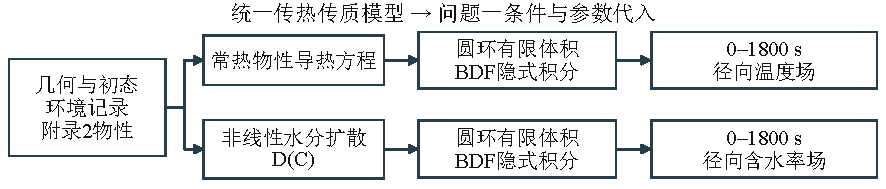
\includegraphics[width=\linewidth]{figures/legibility_schematics/q1_workflow.pdf}
\caption{问题一由统一模型到径向预热模型的求解流程}
\label{fig:q1-workflow}
\end{figure}
\endgroup

\subsection{常热物性方程与初边值条件}
题设圆柱药材长$25\unit{cm}$、半径$2\unit{cm}$。
本问取固定骨架$v_s=0$，式\eqref{eq:heat}、\eqref{eq:moisture}中的材料导数退化为时间偏导数。
初始干密度空间均匀且干物质守恒，故固定骨架下干密度保持均匀，可从水分方程约去。

依假设\ref{ass:midsection}取中截面径向近似并忽略端面影响，以$r,t$描述两场，
计算区间为$0\leq r\leq R$。轴心取零径向梯度，表面通过线性换热、传质关系与环境相联系。
几何与边界条件见图\ref{fig:q1-boundary}。

\begin{figure}[htbp]
\centering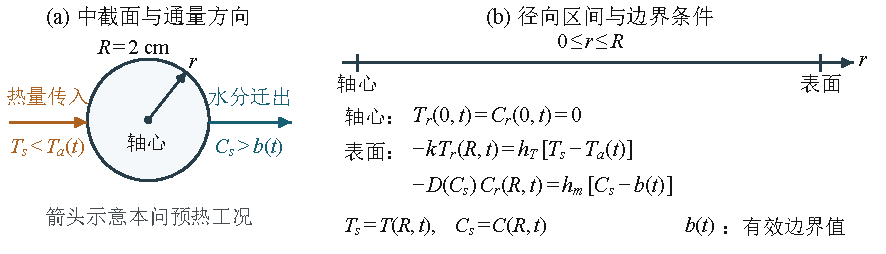
\includegraphics[width=\linewidth]{figures/legibility_schematics/q1_boundary.pdf}
\caption{问题一中截面径向模型与边界条件示意图}
\label{fig:q1-boundary}
\end{figure}

代入附录2的常热物性参数与扩散系数关系，得到径向导热方程与非线性水分扩散方程：
\begin{equation}
\begin{aligned}
T_t&=\alpha\frac{1}{r}\frac{\partial}{\partial r}(rT_r),
&\alpha&=\frac{0.36}{820\times2600},\\
C_t&=\frac{1}{r}\frac{\partial}{\partial r}\bigl(rD(C)C_r\bigr),
&D(C)&=7\times10^{-9}e^{-0.89/C}.
\end{aligned}
\label{eq:q1-pde}
\end{equation}
式\eqref{eq:q1-pde}定义在$0<r<R=0.02\unit{m}$，初态为
$T(r,0)=28\celsius$、$C(r,0)=2.55\unit{kg/kg}$。式\eqref{eq:boundary}
在轴线对称性和圆柱表面外法向下具体写为
\begin{equation}
\begin{aligned}
T_r(0,t)&=C_r(0,t)=0,\\
-0.36T_r(R,t)&=25[T(R,t)-T_a(t)],\\
-D(C_s)C_r(R,t)&=8\times10^{-7}[C_s-b(t)],\qquad C_s=C(R,t).
\end{aligned}
\label{eq:q1-bc}
\end{equation}
其中$T_a,b$由环境记录线性插值得到。本问的$D$不依赖温度，热方程也
不依赖含水率，因此两个场分别求解；水分场仍是非线性的，因为其散度
展开后为$D(C)(C_{rr}+C_r/r)+D'(C)C_r^2$，不能按常扩散率处理。
均匀初态与式\eqref{eq:q1-bc}在初始表面角点不相容，故保留题给初值，
允许$t>0$形成早期边界层，不人为调整初始表面含水率。

\subsection{圆环守恒离散与隐式求解}
为同时说明两个场的计算，记$u=T$时$a(u)=\alpha$、
$\beta=25/(820\times2600)$、$u_a=T_a$；$u=C$时$a(u)=D(u)$、
$\beta=8\times10^{-7}$、$u_a=b$。取节点$r_i=i\Delta r$，
$i=0,\ldots,N$、$\Delta r=R/N$，内部控制体面位于相邻节点中点，
两端面分别为$r_{-1/2}=0$、$r_{N+1/2}=R$。令外向加权通量
$G=-ra(u)u_r$，将式\eqref{eq:q1-pde}乘$r$并在圆环控制体内积分，得
\begin{equation}
\frac{\dd}{\dd t}\int_{r_{i-1/2}}^{r_{i+1/2}}ru\,\dd r
=G(r_{i-1/2},t)-G(r_{i+1/2},t).
\label{eq:q1-ring}
\end{equation}
真实体积中的公因子$2\pi L$已约去。以节点值近似式\eqref{eq:q1-ring}
的储存量，权重为$w_i=(r_{i+1/2}^2-r_{i-1/2}^2)/2$，因此轴心和
表面节点均保留各自控制体容量。把相邻两半格的扩散阻力串联相加，
即$\Delta r/\widehat a=(\Delta r/2)/a(u_i)+(\Delta r/2)/a(u_{i+1})$，
内部面得到调和平均及通量：
\begin{equation}
\widehat a_{i+1/2}=\frac{2a(u_i)a(u_{i+1})}{a(u_i)+a(u_{i+1})},\qquad
G_{i+1/2}=r_{i+1/2}\widehat a_{i+1/2}\frac{u_i-u_{i+1}}{\Delta r}.
\label{eq:q1-flux}
\end{equation}
同一式\eqref{eq:q1-flux}同时用于相邻两格，结合式\eqref{eq:q1-bc}
即得到实际积分的常微分方程组
\begin{equation}
\begin{aligned}
w_i\dot u_i&=G_{i-1/2}-G_{i+1/2},\qquad i=0,\ldots,N,\\
G_{-1/2}&=0,\qquad G_{N+1/2}=R\beta(u_N-u_a).
\end{aligned}
\label{eq:q1-ode}
\end{equation}
轴心内面通量自然为零，式\eqref{eq:q1-ode}无须计算奇异的$1/r$。
逐格求和后内部面通量抵消，由$\sum_iw_i=R^2/2$可得
\begin{equation}
\frac{\dd}{\dd t}\left(\frac{2}{R^2}\sum_{i=0}^Nw_i u_i\right)
=-\frac{2\beta}{R}(u_N-u_a).
\label{eq:q1-balance}
\end{equation}
式\eqref{eq:q1-balance}把圆柱加权平均的变化与表面交换直接对应，
也是数值程序累计边界通量、检查离散总量一致性的依据。

将式\eqref{eq:q1-ode}写为$\dot{\boldsymbol u}=\boldsymbol F(t,\boldsymbol u)$，
使用自适应隐式BDF方法\cite{scipy}。每步的新状态由隐式残量及Newton修正确定：
\begin{equation}
\begin{aligned}
\boldsymbol{\mathcal R}(\boldsymbol u^{n+1})
&=\gamma_n\boldsymbol u^{n+1}-\boldsymbol q_n
-\Delta t_n\boldsymbol F(t_{n+1},\boldsymbol u^{n+1})=\boldsymbol0,\\
\left[\gamma_n I-\Delta t_n J_F\right]\delta\boldsymbol u
&=-\boldsymbol{\mathcal R}.
\end{aligned}
\label{eq:q1-bdf}
\end{equation}
这里$\gamma_n,\boldsymbol q_n$由积分阶数、步长和已知历史状态确定；
实际采用SciPy的变阶BDF实现及其精度修正，式\eqref{eq:q1-bdf}表示共同的
隐式求解结构。解析稀疏Jacobian $J_F=\partial\boldsymbol F/\partial\boldsymbol u$
保留$D'(C)=0.89D(C)/C^2$及调和平均的导数，
在非线性迭代中更新扩散率。积分在每个环境输入折点重启并传递末态。
正式径向区间数为10240，相对容差$2\times10^{-12}$，最大步长$3\unit{s}$；
$1\unit{s}$是输出间隔，不是积分固定步长。

\subsection{规定结果与预热规律}
表\ref{tab:q1-temperature}和表\ref{tab:q1-moisture}给出规定的七个时刻、
五个径向位置。\texttt{result1.xlsx}从第1秒至第1800秒，每隔
$0.1\unit{cm}$输出21个位置的温度和干基含水率，共75600个数值；
计算不提前舍入，输出统一显示四位小数。

\begin{table}[htbp]
\centering\small
\caption{30分钟内药材中截面温度（$^\circ$C）}
\label{tab:q1-temperature}
\input{tables/q1_temperature.tex}
\end{table}

\begin{table}[htbp]
\centering\small
\caption{30分钟内药材中截面干基含水率（kg/kg）}
\label{tab:q1-moisture}
\input{tables/q1_moisture.tex}
\end{table}

$1800\unit{s}$时轴心、表面温度分别为33.5753\celsius{}和
36.7856\celsius，均低于该时刻环境温度41.5130\celsius。表面先响应，
轴心因传导而滞后。由未舍入值计算，径向温差为$3.2102\unit{K}$。
同期表面含水率降至$1.5102\unit{kg/kg}$，轴心实际含水率约为
$2.5499924\unit{kg/kg}$，四位显示仍为2.5500；因此不能把表中轴心数字
未变解释为水分数学上严格不变。

\begin{figure}[htbp]
\centering
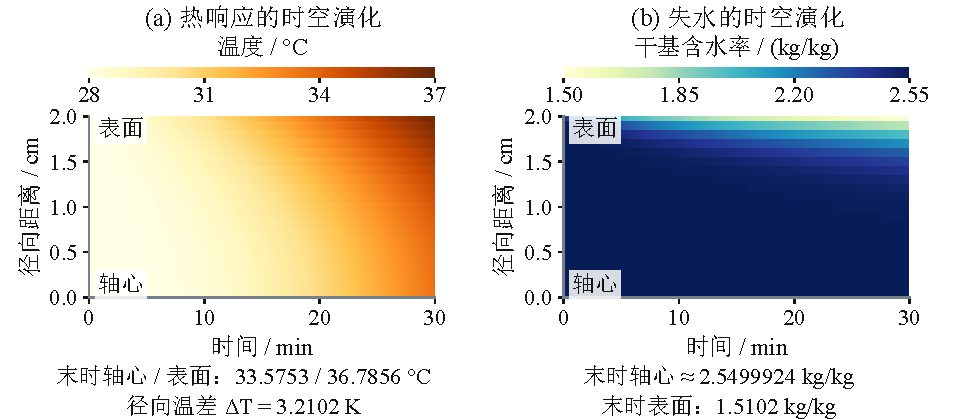
\includegraphics[width=0.94\textwidth]{figures/q1_legibility/q1_profiles.pdf}
\caption{第一问的时间--径向温湿场。横轴为时间，纵轴为径向距离；左、右色标分别表示温度与干基含水率，均由已保存采样值着色。}
\label{fig:q1-profiles}
\end{figure}

\Needspace{3\baselineskip}
沿图\ref{fig:q1-profiles}横向可跟踪同一径向位置的变化，沿纵向可比较同一时刻的内部与表面。色阶显示，升温已遍及所考察的径向位置，而水分变化
主要集中在表层。末时$r=1.5\unit{cm}$处的含水率为2.3755，较初值
下降约6.84\%，$r=1.0\unit{cm}$处仍为2.5383。这里不存在严格截断的
扩散前沿；描述受影响层厚度时需要先规定含水率变化阈值。

\Needspace{3\baselineskip}
以共同尺度$R$比较扩散时间：初始热扩散率
$\alpha=k/(\rho c_p)=1.6886\times10^{-7}\unit{m^2/s}$，
$D(C_0)=4.9377\times10^{-9}\unit{m^2/s}$，故
$R^2/\alpha=2368.89\unit{s}$、$R^2/D(C_0)=81010.11\unit{s}$，
两者相差34.20倍。这解释了预热阶段热响应快于水分响应；因失水使$D$
继续减小，初始扩散时间不是最终烘干时长。
圆柱平均须按$r\,\mathrm dr$加权，得到末时中截面平均温度
35.1679\celsius、平均含水率$2.2936\unit{kg/kg}$；它们不替代最湿点，
也不能直接当作包含端部效应的整根平均量。

\subsection{数值验证与适用范围}
针对前述温湿分布，先以独立参考检验数值一致性。
温度以贝塞尔特征函数展开作参考；
水分经$x=(r/R)^2$变换，以Chebyshev配点与非线性表面条件消元构造独立空间参考解。
正式解与参考解在全部规定输出点上的最大温度差为
$7.29\times10^{-9}\unit{K}$，含水率差为
$1.52\times10^{-6}\unit{kg/kg}$；全部75600个正式输出四位一致。

再检查时间积分精度的影响。固定正式网格收紧时间控制后，温湿差分别约
$5.03\times10^{-10}\unit{K}$和$8.15\times10^{-11}\unit{kg/kg}$。
接近舍入分界的数值必须逐项核对，不能仅凭最大误差小于半个末位单位
推断整张表四位一致。

为进一步检验忽略端面影响后的中截面径向近似，采用同物理条件下的$80\times128$有限圆柱二维模型进行配对比较。
在前$1800\unit{s}$已检查采样点上，中截面的最大温湿差分别约为
$5.65\times10^{-8}\unit{K}$与$4.09\times10^{-9}\unit{kg/kg}$，
支持本问中截面径向近似；端面局部差仍可较大，不能据此推广到整个圆柱。

独立核对与中截面配对为前述温湿分布提供了所选有效方程下的数值依据，
不消除等效湿度边界、参考密度
及无显式潜热假设引入的物理不确定性。
本问预热段的相变能量缺口量级显著，相关诊断与解释范围见第\ref{sec:limitations}节。
\FloatBarrier
\endgroup

\FloatBarrier
\section{问题二：变物性热质耦合与全过程输出}
\label{sec:q2}

\begingroup
% Local white-space settings; body fonts, leading and margins are unchanged.
\setlength{\parskip}{0pt}
\setlength{\abovedisplayskip}{4pt}
\setlength{\belowdisplayskip}{4pt}
\setlength{\abovedisplayshortskip}{4pt}
\setlength{\belowdisplayshortskip}{4pt}
\setlength{\intextsep}{6pt}
\setlength{\textfloatsep}{6pt}
\setlength{\floatsep}{6pt}
\captionsetup{skip=5pt}
\renewcommand{\arraystretch}{1.08}
问题二在第\ref{sec:common-model}章统一模型基础上，采用附录3变物性，从共同初态
联立求解固定半径下的径向温湿场。通过温度与含水率对物性的反馈，
给出规定结果及所设环境延拓下的全程轨迹，为问题三判定终点提供基础。
求解流程见图\ref{fig:q2-workflow}。

\begin{figure}[H]
\centering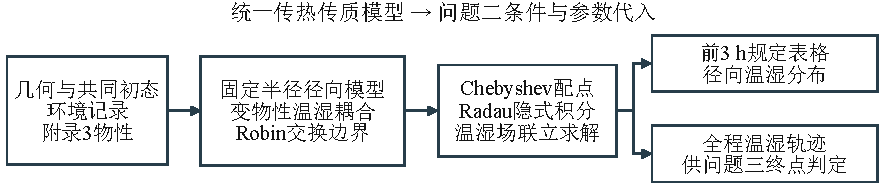
\includegraphics[width=\linewidth]{figures/legibility_schematics/q2_workflow.pdf}
\caption{问题二由统一模型到变物性热质耦合模型的求解流程}
\label{fig:q2-workflow}
\end{figure}

\subsection{从通用方程到变物性耦合系统}
第二问从共同初态开始，全程使用附录3物性，不接续第一问
末态，也不在$1800\unit{s}$处切换公式。有效热容量
$S(C)=\rho_{\rm eff}(C)c_p(C)$和导热率随局部含水率改变，扩散率同时
依赖局部绝对温度$T_K=T+273.15$和$C$。升温改变扩散，失水又通过热容量
及导热率反馈温度，因此需联立推进两个场。

将表\ref{tab:properties}的第二问参数写成
\begin{equation}
\begin{aligned}
S(C)&=(650+128C)\left(1450+\frac{2736C}{1+C}\right),
& k(C)&=0.21+\frac{0.38C}{1+C},\\
D(T,C)&=A(T)e^{-0.45/C},
& A(T)&=2.4\times10^{-3}e^{-3850/T_K}.
\end{aligned}
\label{eq:q2-coefficients}
\end{equation}
固定骨架给出$v_s=0$，空间均匀的参考干密度可从式\eqref{eq:moisture}
约去。再将式\eqref{eq:heat}、\eqref{eq:moisture}的散度取为圆柱径向形式，得
\begin{equation}
\begin{aligned}
T_t&=\frac{1}{rS(C)}\partial_r\!\left[rk(C)T_r\right],\\
C_t&=\frac1r\partial_r\!\left[rA(T)e^{-0.45/C}C_r\right],
\qquad 0<r<R_0.
\end{aligned}
\label{eq:q2-radial}
\end{equation}
例如第一式展开为$T_t=(k/S)(T_{rr}+T_r/r)+(k'(C)/S)C_rT_r$，
显式给出含水率梯度对导热的反馈；不能将其改成
$\nabla\cdot[(k/S)\nabla T]$，否则会额外引入$S$的空间导数。
这里经验$\rho_{\rm eff}(C)$仅用于有效热容量，不同时充当固定体积下
满足真实组成守恒的湿体密度。初态为$T=28\celsius$、$C=2.55$，
轴线零梯度和表面交换沿用式\eqref{eq:boundary}。

\subsection{坐标变换、表面闭合与联合积分}
为避免直接计算$r=0$处的$1/r$，令$x=(r/R_0)^2$。对任意光滑径向场
$v$及系数$a$，由链式法则得到
\begin{equation}
\partial_r=\frac{2r}{R_0^2}\partial_x,\qquad
\frac1r\partial_r(ra\partial_rv)
=\frac4{R_0^2}\partial_x(xa\partial_xv).
\label{eq:q2-coordinate}
\end{equation}
有限的$v_x$自动满足轴线$v_r=0$，且$x=0$处右端取
$4a(0)v_x(0)/R_0^2$，无需人为设置一个很小的替代半径。
按式\eqref{eq:primitive}取$U(C)=\int_0^C e^{-0.45/s}\dd s$，
则$U'(C)=e^{-0.45/C}>0$，水分通量中的$D C_x$恰好等于$A(T)U_x$。
这保留局部温度依赖，并使求导作用于较平缓的原函数场。

在$x_j=[1-\cos(j\pi/N)]/2$，$j=0,\ldots,N$上插值，
记$\mathsf D_x=(\ell'_j(x_i))$为Lagrange插值求导矩阵，
$\mathsf X=\operatorname{diag}(x_j)$；$\mathsf D_x$与物性扩散率$D$含义不同。
对包含表面的节点向量，令
$\boldsymbol q_T=\operatorname{diag}(k_j)\mathsf D_x\boldsymbol T$、
$\boldsymbol q_C=\operatorname{diag}(A_j)\mathsf D_x\boldsymbol U$。
由$\partial_x(xq)=q+xq_x$逐项配点，得到实际采用的半离散系统
\begin{equation}
\begin{aligned}
\dot{\boldsymbol T}_{I}
&=\frac4{R_0^2}
 \left[\operatorname{diag}(S_j^{-1})
 (\mathsf I+\mathsf X\mathsf D_x)\boldsymbol q_T\right]_{I},\\
\dot{\boldsymbol C}_{I}
&=\frac4{R_0^2}
 \left[(\mathsf I+\mathsf X\mathsf D_x)\boldsymbol q_C\right]_{I},
\qquad I=\{0,\ldots,N-1\}.
\end{aligned}
\label{eq:q2-semidscrete}
\end{equation}
其中$\mathsf I$是单位矩阵，下标$I$表示取待积分节点；表面$j=N$
不另设演化方程。由式\eqref{eq:boundary}及$\partial_r=(2/R_0)\partial_x$
在表面联立求解
\begin{equation}
\begin{aligned}
\gamma k(C_s)(\mathsf D_x\boldsymbol T)_N+h_T(T_s-T_a)&=0,\\
\gamma A(T_s)(\mathsf D_x\boldsymbol U)_N+h_m(C_s-b)&=0,
\qquad\gamma=\frac2{R_0}.
\end{aligned}
\label{eq:q2-robin}
\end{equation}
两式的正号来自将外向Robin通量移至同一侧。由于求导矩阵的行和为零，
记$g_T=\sum_{j<N}(\mathsf D_x)_{Nj}(T_j-T_a)$，第一式可消去表面温度：
\begin{equation}
T_s(C_s)=T_a-
\frac{\gamma k(C_s)g_T}{\gamma k(C_s)(\mathsf D_x)_{NN}+h_T}.
\label{eq:q2-surface-elimination}
\end{equation}
代入第二式便得到关于$C_s>0$的一个非线性方程，用阻尼Newton法求根，
再回代$T_s$。因此每次内部状态改变都会同步更新表面温湿，不能分别
指定二者或用上一时刻的表面值替代；时间积分Jacobian也包含这一隐式响应。

将式\eqref{eq:q2-semidscrete}记为$\dot{\boldsymbol y}=\boldsymbol F(t,\boldsymbol y)$，
其中$\boldsymbol y=(T_0,C_0,\ldots,T_{N-1},C_{N-1})^{\mathsf T}$。
采用三阶段Radau隐式积分\cite{scipy}，每步联立求解阶段状态并更新：
\begin{equation}
\begin{aligned}
\boldsymbol Y_i&=\boldsymbol y_n+\Delta t\sum_{j=1}^3
a_{ij}\boldsymbol F(t_n+c_j\Delta t,\boldsymbol Y_j),\quad i=1,2,3,\\
\boldsymbol y_{n+1}&=\boldsymbol y_n+\Delta t\sum_{i=1}^3
b_i\boldsymbol F(t_n+c_i\Delta t,\boldsymbol Y_i).
\end{aligned}
\label{eq:q2-radau}
\end{equation}
$a_{ij},b_i,c_i$为该方法的固定系数；每个阶段均调用上述表面闭合，
式\eqref{eq:q2-radau}从而在同一步内处理温度与含水率反馈。

\subsection{全过程输出与规定结果}

前$4\unit{h}$采用附件1分段线性环境，之后按统一假设保持末小时61点
算术均值：$T_a=49.9989344262\celsius$、$b=0.04998754098$。
第二问与第三问采用同一条温湿联合轨迹，积分至第三问执行端点
$206906.76\unit{s}$，即$57.4741\unit{h}$。因此第二问的完整结果
覆盖所选模型下的全过程，题设表3、表4对应的表\ref{tab:q2-temperature}、\ref{tab:q2-moisture}仅展示前$3\unit{h}$。
环境平台是超出观测范围的假设，不能将此完整时间覆盖称为数天实测验证。

全程轨迹采用80阶Chebyshev配点、原函数形式水分通量和Radau隐式
时间积分，表面温湿由Robin条件联合确定；相对容差$2\times10^{-13}$，
最大步长$30\unit{s}$，前$4\unit{h}$限制为$20\unit{s}$。
\texttt{result2.xlsx}包含两张表，每表从1秒起保存206907个时刻，即
整数秒至206906秒并追加206906.76秒；21个规定半径合计8,690,094个
温湿数值。逐秒评价联合连续解，不将不同模型的温度、水分拼接。

\subsection{规定表格及空间规律}
\begin{table}[!htb]
\centering\small
\caption{3小时内药材中截面温度（$^\circ$C）}
\label{tab:q2-temperature}
\input{tables/q2_temperature.tex}
\end{table}

\begin{table}[!htb]
\centering\small
\caption{3小时内药材中截面干基含水率（kg/kg）}
\label{tab:q2-moisture}
\input{tables/q2_moisture.tex}
\end{table}

至$3\unit{h}$，轴心、表面温度分别为49.8495\celsius、49.9664\celsius，
相差$0.1169\unit{K}$；含水率分别为1.7662、1.0081，相差
$0.7581\unit{kg/kg}$。温度接近空间均匀时，水分仍有明显梯度，
不能用均匀含水率的集中参数近似替代径向场。
按$r\,\mathrm dr$加权，平均温度为49.9043\celsius，平均含水率为
$1.3825\unit{kg/kg}$，相对初始含水率下降45.7833\%。该比例是固定参考
干密度下的有效水分减少比例，不是实测总质量损失率。

\begin{figure}[!htb]
\centering
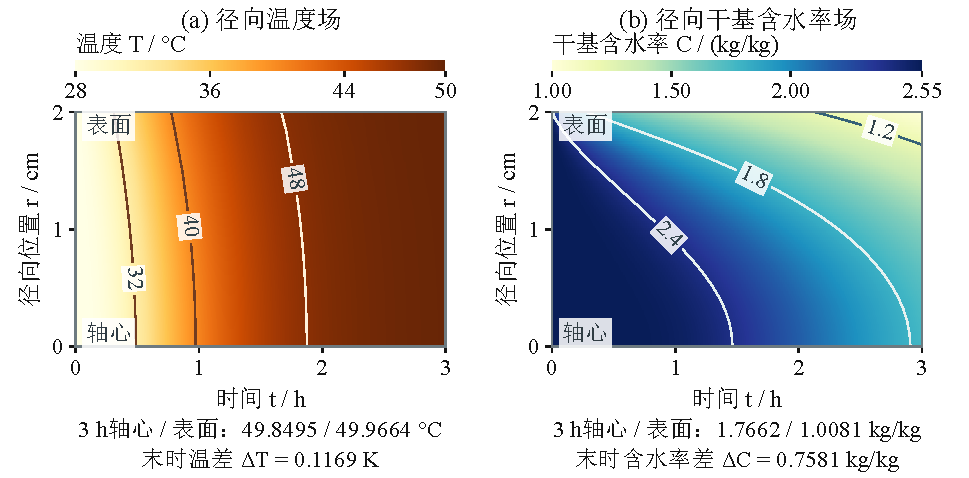
\includegraphics[width=0.94\textwidth]{figures/legibility_q2/q2_fields.pdf}
\caption{第二问前3小时径向温度场与干基含水率场的时空演化。横轴为时间，纵轴为径向位置，颜色表示场量大小；等值线辅助辨识时空分布，末时径向差值另作标注。}
\label{fig:q2-profiles}
\end{figure}

图\ref{fig:q2-profiles}左图显示温度总体随时间升高，并逐渐趋于径向均匀；
右图显示含水率先在表层下降，低含水区域随后向内部扩展，径向差异仍较明显。

第二问$0.5\unit{h}$轴心温度32.1892\celsius，低于第一问同一
时刻；这是从初态使用不同物性、尤其初始有效热容量更大的正常结果，
不是问间接口错误。第一问和第二问是不同参数情形，不能共用一段预热轨迹。

\subsection{升温促进与失水抑制的竞争}
将附录3扩散系数相对初态取对数，可精确分解为
\begin{equation}
\begin{aligned}
\ln\frac{D(t,r)}{D_0}&=H(t,r)+M(t,r),\\
H&=3850\left(\frac1{301.15}-\frac1{T_K}\right),\qquad
M=0.45\left(\frac1{2.55}-\frac1C\right).
\end{aligned}
\label{eq:q2-log-mechanism}
\end{equation}
其中$D_0=5.64168037\times10^{-9}\unit{m^2/s}$。
$H$度量沿当前轨迹的累计温度贡献，$M$度量累计含水率贡献；这是代数
分解，不能当作独立改变某一因素的因果贡献百分比。

图\ref{fig:q2-mechanism}展示上述分解；前$3\unit{h}$逐秒采样中，轴心与表面扩散率
分别于约$2.46\unit{h}$和$2.02\unit{h}$达到该时段的采样峰值，随后回落。

\begin{figure}[htbp]
\centering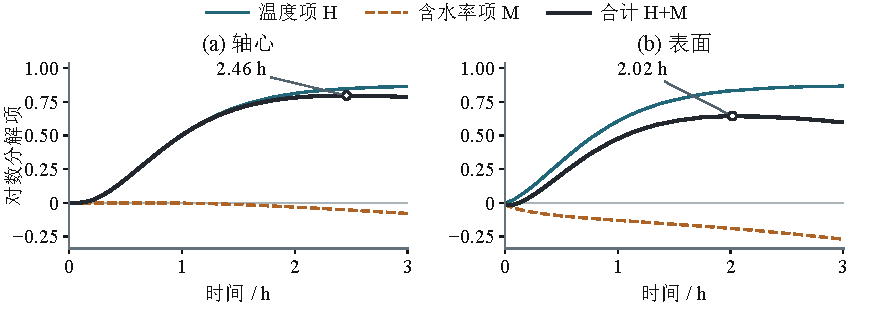
\includegraphics[width=\linewidth]{figures/legibility_q2/q2_mechanism.pdf}
\caption{第二问前3小时轴心与表面的扩散率对数分解。$H$为温度贡献，$M$为含水率贡献，$H+M=\ln(D/D_0)$；标记为逐秒采样峰值，不表示连续时间严格极值。}
\label{fig:q2-mechanism}
\end{figure}

$3\unit{h}$时，轴心与表面的$D/D_0$分别为2.1957与1.8207，说明相对
初态累计升温促进仍占优势；但最后半小时，两处扩散率分别下降约1.06\%
和3.16\%。因此“扩散系数全程单调增加”不成立。表面还曾在早期每秒
采样的第144秒达到$D/D_0=0.983282$的局部最低值。温度变化和失水抑制
的竞争随阶段变化，前3小时的累计主导关系不能直接用于判定末期干燥瓶颈。

在同一320区间有限体积网格上单独扰动交换系数，$h_m$降低、提高20\%
时，$3\unit{h}$表面含水率分别为1.1775、0.8737；相应轴心值为1.8581、
1.6921。对这一输出和扰动区间，水分交换系数的影响明显大于数值误差。
该对照为人为情景而非参数置信区间（见第\ref{sec:environment-scenarios}节），
不能替代气固水分基准识别\cite{dasilva2014,adrover2020}。

\subsection{独立验证与适用范围}
以下核查数值输出与模型账本的一致性，并检验降维适用范围。

前3小时已有节点有限体积逐级加密至2560区间及Richardson外推，
另用独立空间离散与Radau积分核对。全程轨迹与该外推轨迹在前3小时
共同采样点的最大温差约$1.07\times10^{-9}\unit{K}$、含水率差约
$8.41\times10^{-8}\unit{kg/kg}$；前3小时温湿表及规定60个论文表值四位一致。
有限体积外推是这一前3小时交叉验证的来源，不是完整工作簿的生成方法。

长时段另与已完成的160阶BDF轨迹在全部60秒采样点及同一执行端点比较，
最大温湿差约$3.27\times10^{-9}\unit{K}$与$9.33\times10^{-9}\unit{kg/kg}$，
四位输出一致。当前869万余格工作簿与同源未舍入轨迹的舍入核对全部通过，
该检查支持导出一致性；高阶独立参考覆盖的是所列采样点，不能把导出
一致性误写成全部逐秒状态均另作了独立求解。

原有限体积有效水分账本的最大残差约$6.51\times10^{-12}\unit{kg/kg}$。
热账本核对的是有效热容量积分与边界热流，即比较
$\int\!\int S(C)T_t\,\mathrm dV\mathrm dt$与累计边界热量，
相对残差约$3.11\times10^{-11}$，并非$\int ST\,\mathrm dV$的末初差，
更不构成潜热、携焓及真实总能量已经闭合的证明。
同物理$80\times256$二维配对在前3小时已检查采样点的中截面最大温湿差
约为$1.692\times10^{-3}\unit{K}$、$2.247\times10^{-5}\unit{kg/kg}$。
这支持中截面的工程近似，但不能保证降维后所有四位显示相同；长期全域
达标须结合第三问终点证据，不能直接沿用前3小时的几何误差。
本问早期大通量阶段亦受相变能量缺口约束，相关量级诊断与闭合限制见第\ref{sec:limitations}节。

综上，温湿场响应不同步，升温促进与失水抑制呈阶段性竞争；
所得同一条轨迹为问题三追踪径向最大含水率、判定干燥终点提供计算基础。
\FloatBarrier
\endgroup

\FloatBarrier
\section{问题三：由全域含水率约束确定干燥时长}
\label{sec:q3}

\begingroup
% Local spacing accommodates the added introduction without changing text size.
\setlength{\parskip}{2pt plus 1pt minus 1pt}
\setlength{\abovedisplayskip}{8pt plus 2pt minus 2pt}
\setlength{\belowdisplayskip}{8pt plus 2pt minus 2pt}
\setlength{\abovedisplayshortskip}{6pt plus 2pt minus 1pt}
\setlength{\belowdisplayshortskip}{6pt plus 2pt minus 1pt}
问题三在问题二变物性热质耦合模型的基础上，进一步确定满足含水率要求的干燥时长。
本问保持控制方程、物性关系与环境边界不变，沿用同一初态下的温湿联合轨迹。
在一维径向模型中，以全径向最大含水率严格低于$0.15\unit{kg/kg}$为终止要求，
不以表面含水率或截面平均值代替最大值。先通过下降穿越检测与括区求根定位候选等号根，
再以径向重构极值复核；结合网格加密和独立积分对照设置经验数值余量，
选取并复核严格满足阈值要求的执行点，给出所设环境条件下的模型干燥时长与径向含水率分布。
求解流程见图\ref{fig:q3-workflow}。

\begingroup
\setlength{\intextsep}{10pt}
\begin{figure}[H]
\centering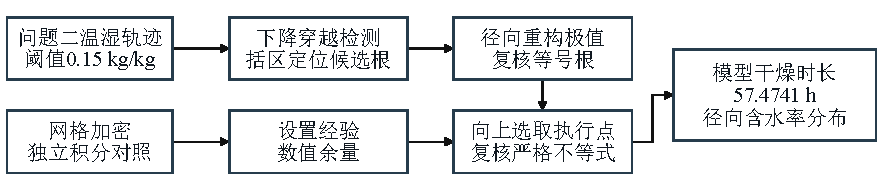
\includegraphics[width=\linewidth]{figures/q3_white/q3_workflow.pdf}
\caption{问题三的一维径向终点判定流程}
\label{fig:q3-workflow}
\end{figure}
\endgroup

\subsection{终止判据与长时计算}

问题三要求药材各处的干基含水率严格低于
$C_{\mathrm{lim}}=0.15\unit{kg/kg}$。
本文沿用问题二的附录3物性、初态和环境条件，
由同一温湿联立轨迹确定终点，而不以表面含水率或截面平均值代替最大值。
因此，本问直接沿用式\eqref{eq:q2-radial}的控制方程及
式\eqref{eq:q2-semidscrete}、\eqref{eq:q2-robin}的离散闭合，
新增的求解任务是从时间轨迹中定位满足全径向约束的执行点。
在一维径向近似中定义
\begin{equation}
 M_1(t)=\max_{0\le r\le R_0}C(r,t),\qquad
 M_1(t_{*,3})=C_{\mathrm{lim}}.
 \label{eq:q3-event}
\end{equation}
所取事件为结束附近的下降穿越。
等号根是严格达标时间集合的边界，根本身不满足题设严格不等式；
有限圆柱中“各处”的含义则由后述二维计算另行检验。

附件1仅覆盖前4\unit{h}，长时计算需延拓环境。
本文保持前述末小时61点算术均值平台，
即环境温度49.9989344262\celsius、有效边界值
$b=0.04998754098\unit{kg/kg}$。
该平台是假设的后续工况，不是4\unit{h}以后的观测记录。
温度和含水率始终按式\eqref{eq:heat}--\eqref{eq:boundary}联立推进，
不在温度接近环境后直接将温度场替换为常数。

随着含水率降低，扩散系数中的
$\exp(-0.45/C)$迅速减小，长时低含水率阶段需要保留局部非线性通量。
令
\begin{equation}
 \begin{aligned}
 a_3(T)&=2.4\times10^{-3}
 \exp\!\left[-\frac{3850}{T+273.15}\right],\\
 F_3(C)&=\int_0^C\exp(-0.45/s)\,\dd s,\qquad
 D\nabla C=a_3(T)\nabla F_3(C).
 \end{aligned}
 \label{eq:q3-primitive}
\end{equation}
采用80阶Chebyshev配点和隐式Radau方法推进，表面状态由Robin条件联立确定。
式\eqref{eq:q3-primitive}只改写通量，不改变题给扩散系数。
临界附近同时检查径向重构极值和边界值，确认最大含水率位于轴心。
空间加密与不同隐式时间方法作为交叉核验，
规定表格和完整结果均由同一未舍入轨迹生成。

\subsection{由重构空间极值到时间事件}

令$P_U(x,t)=\sum_{j=0}^N F_3(C_j(t))\ell_j(x)$为包含表面状态的
原函数插值多项式，$x=(r/R_0)^2$。在$P_U>0$的物理解支上，含水率重构为
$C_N(x,t)=F_3^{-1}[P_U(x,t)]$。由于$F_3'(C)>0$，
有$\partial_x C_N=\partial_xP_U/F_3'(C_N)$，故两者的内部驻点相同。
每一时刻的极值候选集为
\begin{equation}
 \mathcal X(t)=\{0,1\}\cup
 \{x\in(0,1):\partial_xP_U(x,t)=0\}.
 \label{eq:q3-extrema-candidates}
\end{equation}
求出式\eqref{eq:q3-extrema-candidates}中的全部实根，并比较候选点值，得到
\begin{equation}
 \widehat M_1(t)=\max_{x\in\mathcal X(t)}C_N(x,t)
 =F_3^{-1}\!\left[\max_{x\in\mathcal X(t)}P_U(x,t)\right].
 \label{eq:q3-reconstructed-max}
\end{equation}
该式确定的是重构一维场的最大值；重构误差及与连续方程的差异仍需
数值加密检验，不能把多项式极值的求全等同于连续模型严格误差为零。

实际程序先以内部节点事件$g_{\rm node}(t)=\max_{j<N}C_j(t)-C_{\rm lim}$
检测下降穿越。当相邻接受步满足
$g_{\rm node}(t_a)>0$、$g_{\rm node}(t_b)\le0$时，利用Radau的步内连续插值
对$g_{\rm node}(t)=0$作Brent括区求根，再在候选根和执行点按
式\eqref{eq:q3-reconstructed-max}复核，并用根两侧节点值检查下降穿越。
本算例确认根与执行点的重构最大值均位于轴心，节点候选根才可用于所述径向终点。
若重构出现更湿的内部点，就必须重新定位事件，不能直接接受节点根。

为解释时间裕量的尺度，在根附近作一阶展开：
\begin{equation}
 \widehat M_1(t_*+\delta t)-C_{\rm lim}
 \approx\dot{\widehat M}_1(t_*)\,\delta t,
 \qquad
 |\delta t|\approx\frac{|\delta M|}{|\dot{\widehat M}_1(t_*)|}.
 \label{eq:q3-local-event-scale}
\end{equation}
这里$\delta M$为含水率的局部数值差。已有事件记录给出末期斜率约
$-2.9128\times10^{-7}\unit{(kg/kg)/s}$；因此显示到四位小数的0.1500
不能支持亚秒级的达标判定。式\eqref{eq:q3-local-event-scale}仅作局部误差尺度
解释，正式时间预算仍取自网格与时间方法对照，不能由该线性近似给出严格界。

\subsection{结束时长与径向水分分布}

一维模型的临界根为
$t_{*,3}=206906.389932328\unit{s}$，即约57.4739972\unit{h}。
为区分数值根、执行点和四位小时显示值，
取显示时间量子$\Delta t=0.0001\unit{h}=0.36\unit{s}$，
并按空间、时间及独立方法差异设置
$\varepsilon_{t,3}=0.03\unit{s}$的经验数值余量，选择
\begin{equation}
 t_{\mathrm{exec},3}
 =\Delta t\left\lceil
 \frac{t_{*,3}+\varepsilon_{t,3}}{\Delta t}\right\rceil
 =206906.76\unit{s}
 =\boxed{57.4741\unit{h}}.
 \label{eq:q3-execution}
\end{equation}
在该实际时刻重新代入未舍入一维场，得到
\begin{equation}
 M_1(t_{\mathrm{exec},3})
 =0.149999892208\unit{kg/kg}<0.15\unit{kg/kg}.
 \label{eq:q3-end-moisture}
\end{equation}
执行点比临界根晚约0.3701\unit{s}。
这里的经验余量用于当前方程的数值选择，
不含环境、边界映射和物性假设的不确定性，也不是实验安全上界。

题设表5要求的每6\unit{h}及结束时刻的径向含水率见表\ref{tab:q3-moisture}。
18\unit{h}时，表面已降至0.0845\unit{kg/kg}，
轴心仍为0.2988\unit{kg/kg}；54\unit{h}时轴心仍为0.1539\unit{kg/kg}。
因此，表面先达到要求并不能作为全体材料的终止依据。
末期水分向低湿表面迁移，而局部扩散系数随含水率下降，
共同形成中心缓慢趋近阈值的尾段。

\begin{table}[htbp]
 \centering
 \caption{题设表5：固定半径时的径向干基含水率（\unit{kg/kg}）}
 \label{tab:q3-moisture}
 \small
 \input{tables/q3_moisture.tex}
\end{table}

完整的\texttt{result3.xlsx}以60\unit{s}为间隔、0.1\unit{cm}为径向间隔输出，
并在最后一个完整分钟206880\unit{s}之后补入执行点206906.76\unit{s}。
末行轴心显示为0.1500，是式\eqref{eq:q3-end-moisture}的四位舍入值；
达标判断使用未舍入场而不使用表格显示值。
160阶空间加密参考和另一隐式时间方法在全部72429个规定水分输出上四位一致，
\mbox{其中空间加密参考}与正式轨迹的最大未舍入差约
$9.33\times10^{-9}\unit{kg/kg}$。
该结果支持已选方程的数值稳定性，不替代物理参数验证。

\begin{figure}[htbp]
 \centering
 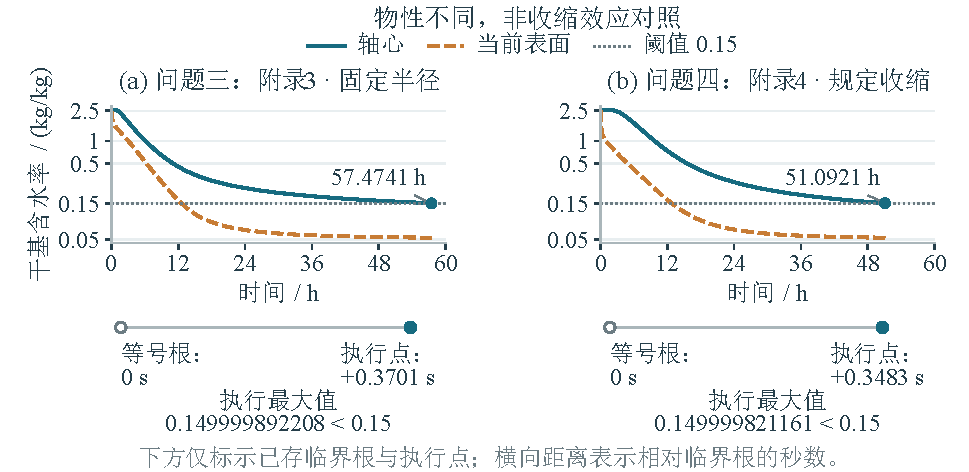
\includegraphics[width=0.93\textwidth]{figures/legibility_process/q3_q4_drying.pdf}
 \caption{问题三（左）与问题四（右）的干燥过程与事件判定。上排为一维径向有效模型的轴心、当前表面含水率演化。
 纵轴为对数刻度，水平线为0.15\unit{kg/kg}阈值，终点标记对应各自正式执行时刻。
 下排以各自临界根为时间原点，仅标示已存临界根与执行点，并列出执行最大值。
 两问采用各自附录物性，问题四另施加观测半径历程，
 因而曲线差异不能全部归因于收缩。}
\label{fig:q3-q4-drying}
\end{figure}

图\ref{fig:q3-q4-drying}上排展示表面先失水、轴心控制尾段的过程；下排将等号临界根与已选执行点分开，时间差直接取自原事件记录。

\subsection{有限圆柱检验与工况条件}

为检验“各处”的空间含义，在长度0.25\unit{m}的有限圆柱上增加轴向传递，
侧面与端面保持相同物性和交换系数。
以80个径向区间、256个轴向区间的同网格一维/二维配对计算比较事件根，
二维比配对一维提前约7.4740\unit{s}。
这一差值用于识别端部效应，不能把粗网格二维绝对根
直接替代精细一维根。

\Needspace{6\baselineskip}
再从临界附近已保存的二维场推进至式\eqref{eq:q3-execution}的执行时刻，
得到全节点最大含水率$0.149998606290\unit{kg/kg}$，
最湿点位于中截面轴心，离散场已经达标。
该节点结果与配对根差支持$57.4741\unit{h}$的工程保守方向；
局部续算仍继承前史离散误差，尚不构成连续二维域的严格数学误差界，
也不将该时长解释为精确的二维最短时间。
上述证据层级集中见第\ref{sec:limitations}节。

后段环境对终时的影响大于末位数值差。
例如，在相同4\unit{h}初始全场和其余参数下，
将之后温度平台降低1\unit{K}，事件根由约57.4740\unit{h}延至59.3413\unit{h}；
升高1\unit{K}则变为55.6884\unit{h}。
该单因素情景为人为设定而非观测误差范围（见第\ref{sec:environment-scenarios}节）。
故57.4741\unit{h}应与环境平台和有效气固边界共同报告，
不能仅凭小数位数给出真实工况下的确定性保证。

\endgroup

\FloatBarrier
\section{问题四：观测收缩下的干燥过程}
\label{sec:q4}

\begingroup
% Local display spacing accommodates the introduction; text and figure sizes are unchanged.
\setlength{\abovedisplayskip}{8pt plus 2pt minus 2pt}
\setlength{\belowdisplayskip}{8pt plus 2pt minus 2pt}
\setlength{\abovedisplayshortskip}{6pt plus 2pt minus 1pt}
\setlength{\belowdisplayshortskip}{6pt plus 2pt minus 1pt}
问题四在第\ref{sec:common-model}章统一模型基础上，结合附件2的观测半径，
在恒长度、均匀径向收缩假设下，用材料坐标与干物质守恒处理几何变化。
采用附录4物性，从共同初态联立求解温湿场，沿用问题三的径向最大含水率判据
确定所设环境条件下的模型干燥时长，并通过同物性恒半径对照分析收缩作用。
求解流程见图\ref{fig:q4-workflow}。

\begingroup
\setlength{\intextsep}{10pt}
\begin{figure}[H]
\centering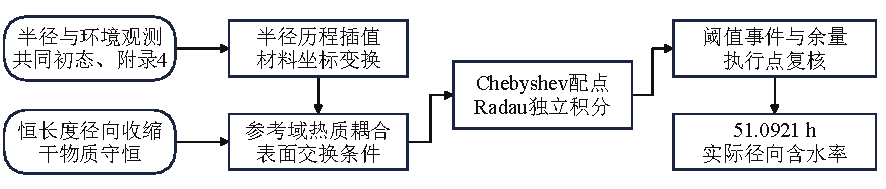
\includegraphics[width=\linewidth]{figures/legibility_schematics/q4_workflow.pdf}
\caption{问题四的收缩模型求解流程}
\label{fig:q4-workflow}
\end{figure}
\endgroup

\subsection{半径历程与材料运动}

问题四将附录4物性代入式\eqref{eq:heat}--\eqref{eq:boundary}，
并根据附件2把固定几何改为运动材料域。
温度和含水率从28\celsius、2.55\unit{kg/kg}的共同初态重新求解，
不接续问题三的干燥末态。
附件2含0--72\unit{h}的145个半径记录，间隔1800\unit{s}，
半径由2\unit{cm}降至1.198\unit{cm}。
本文将半径转换为米后分段线性插值为$R(t)$，
保持其单调性和平台段；所求主终点位于观测时域内。
环境继续采用前4\unit{h}观测插值及之后的共同均值平台。

外半径只规定边界位置，不能唯一确定内部材料运动。
采用均匀径向收缩、长度$L=L_0$不变的运动学闭合，
定义材料标记$\xi$及映射
\begin{equation}
 r=R(t)\xi,\quad z=Z,\qquad
 v_{s,r}=\frac{R'(t)}{R(t)}r=w_r,\quad v_{s,z}=0,
 \qquad J=\left(\frac{R(t)}{R_0}\right)^2.
 \label{eq:radius-map}
\end{equation}
其中$w_r=\partial r/\partial t|_\xi$为网格速度，$J$为体积Jacobian。
该材料映射是一项附加假设，而不是半径记录直接测得的内部变形。
移动边界模型须区分体积水浓度与材料干基含水率，
并以当前界面的相对通量写守恒条件\cite{adrover2020}。

\subsection{干基守恒与参考域方程}

当前体积水浓度为$\rho_d C$。
对干物质与水分别写守恒式，并采用相对材料的扩散通量，得
\begin{equation}
 \begin{aligned}
  &\partial_t\rho_d+\nabla\cdot(\rho_d\boldsymbol v_s)=0,\\
  &\partial_t(\rho_d C)
   +\nabla\cdot(\rho_d C\boldsymbol v_s+\boldsymbol j_w)=0,
  \qquad \boldsymbol j_w=-\rho_dD\nabla C.
 \end{aligned}
 \label{eq:q4-component-balance}
\end{equation}
第二式减去第一式的$C$倍，即得到式\eqref{eq:moisture}。
由初始干密度均匀和式\eqref{eq:radius-map}，
$\rho_d J=\rho_{d,0}$，所以
$\rho_d(t)=\rho_{d,0}[R_0/R(t)]^2$为空间常数，可从干基水分方程中约去。
对任一场量$f(r,t)=\widehat f(\xi,t)$，链式法则给出
\begin{equation}
 \left.\partial_t f\right|_r
 =\left.\partial_t\widehat f\right|_\xi
   -\frac{R'}R\xi\partial_\xi\widehat f,
 \qquad
 v_{s,r}\partial_r f=\frac{R'}R\xi\partial_\xi\widehat f.
 \label{eq:q4-chain-rule}
\end{equation}
两项中的材料运动恰好抵消，故$\Ds f/\dd t=\partial_t\widehat f|_\xi$。
再将$\partial_r=R^{-1}\partial_\xi$代入式\eqref{eq:heat}和\eqref{eq:moisture}，
省略场量帽号后，一维参考域方程为
\begin{equation}
 \begin{aligned}
  \left.\partial_t C\right|_\xi
   &=\frac{1}{R(t)^2\xi}\partial_\xi
     \left[\xi D(T,C)\partial_\xi C\right],\\
  \rho_{\mathrm{eff}}(C)c_p(C)
   \left.\partial_t T\right|_\xi
   &=\frac{1}{R(t)^2\xi}\partial_\xi
     \left[\xi k(C)\partial_\xi T\right].
 \end{aligned}
 \label{eq:q4-reference-pde}
\end{equation}
轴线取正则对称条件；将同一空间导数变换代入式\eqref{eq:boundary}，
当前侧表面的边界式为
\begin{equation}
 -\frac{D(T_s,C_s)}{R}\left.\partial_\xi C\right|_1=h_m(C_s-b),
 \qquad
 -\frac{k_s}{R}\left.\partial_\xi T\right|_1=h_T(T_s-T_a).
 \label{eq:q4-reference-boundary}
\end{equation}
其中$k_s=k(C_s)$，表面系数均按当前温湿状态计算。

式\eqref{eq:q4-reference-pde}没有额外的几何浓缩源。
无交换的纯收缩使体积水浓度$\rho_d C$增加，
但水与干物质质量均不变，因此干基$C$应保持不变。
若再加入$-2R'C/R$或另一个网格对流项，就会重复计算已经包含的材料运动。
附录$\rho_{\mathrm{eff}}$用于有效热容量，$\rho_d$用于上述质量账本；
二者不能同时通过$\rho_d=\rho_{\mathrm{eff}}/(1+C)$强制等同为真实组分密度。
热式仍无显式潜热，数值闭合不构成真实组分总焓守恒的证明（见第\ref{sec:limitations}节）。

附录4的局部扩散系数为
\begin{equation}
 D(T,C)=4.2\times10^{-4}
 \exp(-0.30/C)
 \exp\!\left[-\frac{3850}{T+273.15}\right].
 \label{eq:q4-diffusivity}
\end{equation}
全部热物性也在各空间位置按当前$C$更新，
温湿两场继续联立求解。
表面交换系数沿用$h_T=25\unit{W/(m^2\cdot K)}$、
$h_m=8\times10^{-7}\unit{m/s}$，
式\eqref{eq:q4-reference-boundary}中的质量通量相对于材料界面，
不另将表面扫过的体积计为蒸发失水。

\subsection{数值求解、账本与结束状态}

令$x=\xi^2$，对任意扩散系数$a$和场量$f$有
\begin{equation}
 \frac{1}{R^2\xi}\partial_\xi(a\xi\partial_\xi f)
 =\frac4{R^2}\partial_x(ax\partial_x f)
 =\frac4{R^2}\bigl[q+x\partial_xq\bigr],
 \qquad q=a\partial_xf.
 \label{eq:q4-x-operator}
\end{equation}
该式消去轴线显式奇点，在$x=0$处直接取$4q(0)/R^2$。
依式\eqref{eq:primitive}定义$F_4'(C)=\exp(-0.30/C)$、$F_4(0)=0$，
并令$A_4(T)=4.2\times10^{-4}\exp[-3850/(T+273.15)]$。
沿用问题二的Chebyshev微分矩阵$\mathsf D_x$，
记$q_{T,i}=k(C_i)(\mathsf D_x\boldsymbol T)_i$、
$q_{C,i}=A_4(T_i)[\mathsf D_x F_4(\boldsymbol C)]_i$
及$S_i=\rho_{\mathrm{eff}}(C_i)c_p(C_i)$，则内部节点方程为
\begin{equation}
 \begin{aligned}
  \dot T_i&=\frac4{R(t)^2S_i}
       \bigl[q_{T,i}+x_i(\mathsf D_x\boldsymbol q_T)_i\bigr],\\
  \dot C_i&=\frac4{R(t)^2}
       \bigl[q_{C,i}+x_i(\mathsf D_x\boldsymbol q_C)_i\bigr].
 \end{aligned}
 \label{eq:q4-semidiscrete}
\end{equation}
其中$i=0,\ldots,N-1$，表面$i=N$由式\eqref{eq:q4-reference-boundary}确定：
\begin{equation}
 \frac2R q_{T,N}+h_T(T_N-T_a)=0,
 \qquad
 \frac2R q_{C,N}+h_m(C_N-b)=0.
 \label{eq:q4-discrete-robin}
\end{equation}
这里$\partial_\xi=2\xi\partial_x$使表面因子成为$2/R$，
而内部演化因子为$4/R^2$；二者均随观测半径更新。
取$N=120$，联立求解表面温湿代数方程后用Radau推进内部未知量，
在环境及半径输入节点处分段重启。

参考圆环的当前体积与固定干质量分别为
$V_i=\pi R^2L_0(\xi_e^2-\xi_w^2)$、$m_{d,i}=\rho_d V_i$。
利用圆环权重与固定干质量构造水量账本\cite{dasilva2014}，有
\begin{equation}
 \overline C(t)=\int_0^1C(x,t)\,dx,
 \qquad
 \overline C(t)+\int_0^t\frac{2h_m}{R(\tau)}
       [C_s(\tau)-b(\tau)]\,d\tau=C_0.
 \label{eq:q4-water-ledger}
\end{equation}
边界通量积分与空间平均的全程段末最大差为
$4.96\times10^{-13}\unit{kg/kg}$。
72\unit{h}零交换纯收缩检验中，温度与干基含水率保持初态，
干物质和水质量的相对变化小于$4.45\times10^{-16}$。
这两项检验针对已选干基守恒与材料运动，
不把经验密度的物理解释也视为已验证。

将配点阶数由120增加至160，共同输出点最大含水率差为
$8.56\times10^{-12}\unit{kg/kg}$；
同阶BDF时间方法与Radau的临界根差约
$5.98\times10^{-4}\unit{s}$。
另用640个径向区间的有限体积独立离散，在相同材料位置比较，
最大含水率差约$1.58\times10^{-5}\unit{kg/kg}$，
最后两级空间外推的根与谱法相差约0.0129\unit{s}。
前两类检验显示谱解已稳定，有限体积外推提供不同离散方法的支持，
外推差仍是经验数值指标而非严格误差界。

终点检测先由内部节点最大值产生等号候选事件，
再将式\eqref{eq:q3-extrema-candidates}--\eqref{eq:q3-reconstructed-max}
中的原函数替换为$F_4$，检查重构多项式的全部内部实驻点及两端点。
由于$F_4'(C)>0$，该检查同时给出重构含水率的最大值；
本算例在候选根和相邻时刻均确认最大值位于轴心。
一维径向极值下降至阈值时，临界根为
$t_{*,4}=183931.211715489\unit{s}$。
根前后1\unit{s}的最大值分别约为0.150000513489和0.149999486518，
最大位置在轴心。
采用$\varepsilon_{t,4}=0.129\unit{s}$的经验数值预算，
按式\eqref{eq:q3-execution}相同的0.36\unit{s}量子向上选择执行点，得
\begin{equation}
 \begin{aligned}
  t_{\mathrm{exec},4}&=183931.56\unit{s}
      =\boxed{51.0921\unit{h}},\\
  \max_{0\le r\le R(t_{\mathrm{exec},4})}C(r,t_{\mathrm{exec},4})
      &=0.149999821161\unit{kg/kg}<0.15\unit{kg/kg}.
 \end{aligned}
 \label{eq:q4-execution}
\end{equation}
该点晚于一维根约0.3483\unit{s}，当前半径为1.2000\unit{cm}。
题设表6的规定采样见表\ref{tab:q4-moisture}。
对规定的实际位置$r_j$，以$P_{U,4}(x,t)$表示$F_4(C)$的配点插值多项式，
导出值按下式由当前材料场重构：
\begin{equation}
 C(r_j,t)=F_4^{-1}\!\left[
 P_{U,4}\!\left(\frac{r_j^2}{R(t)^2},t\right)\right],
 \qquad 0\le r_j\le R(t).
 \label{eq:q4-output-map}
\end{equation}
当$r_j>R(t)$时不作域外外推；当前表面取$x=1$另列，
不能当作固定2\unit{cm}位置。

\begin{table}[H]
 \centering
 \caption{题设表6：收缩过程中的干基含水率（\unit{kg/kg}）}
 \label{tab:q4-moisture}
 \small
 \input{tables/q4_moisture.tex}
\end{table}

表中域外位置以“—”表示不适用，不能解释成零含水率。
\texttt{result4.xlsx}按60\unit{s}、0.1\unit{cm}导出，
并补入实际执行点；域外单元格留空，另保留表面值与当前半径。
末行轴心四位显示0.1500，严格不等式判断仍基于
式\eqref{eq:q4-execution}的未舍入值。

% The result table is anchored above; keep the following figure free to float.
\Needspace{6\baselineskip}
\subsection{收缩作用与模型解释}

\begin{figure}[htbp]
 \centering
 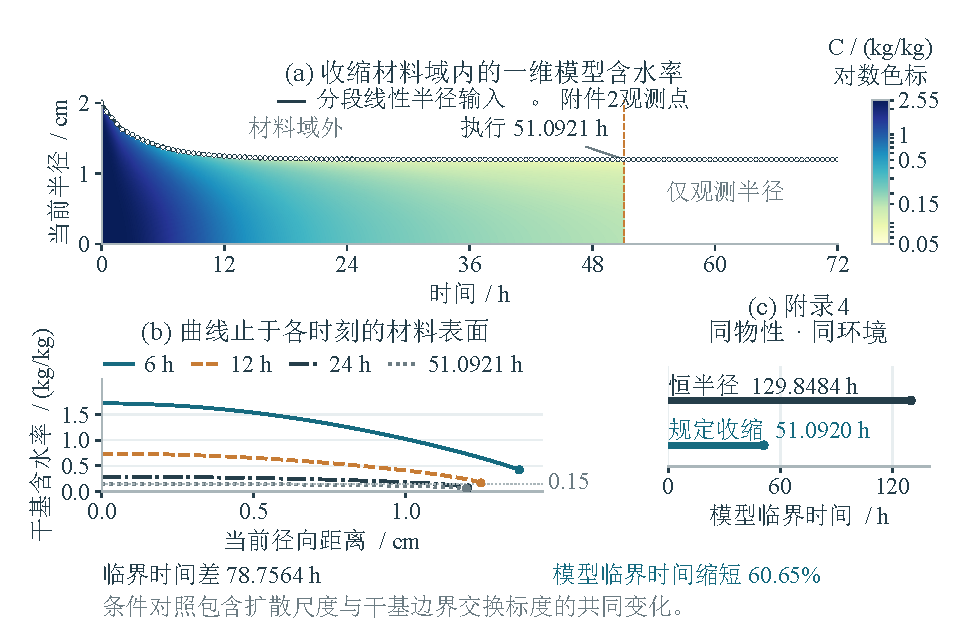
\includegraphics[width=0.92\textwidth]{figures/legibility_process/q4_shrinkage.pdf}
 \caption{规定收缩下的径向有效模型场、观测输入与同物性条件对照。(a)当前实际半径坐标中的含水率色图仅显示至正式执行时刻，采用对数色标；全部观测点及分段线性半径输入保留至72\unit{h}，执行线之后只展示半径。(b)各时刻含水率剖面止于当时材料表面。(c)附录4同物性、同环境下的恒半径与规定收缩临界根对照。临界根与执行时刻分别标示；时间差包含扩散尺度和干基边界交换标度变化。}
 \label{fig:q4-shrinkage}
\end{figure}
\Needspace{3\baselineskip}
图\ref{fig:q4-shrinkage}在当前实际半径坐标中展示规定收缩与含水率演化；上方色图止于正式执行时刻并保留完整半径观测输入，左下剖面止于各时刻的材料表面，右下对照原恒半径与规定收缩的临界时间。
为分离施加收缩历程的作用，另保持附录4和其余条件不变，
将半径固定为2\unit{cm}作受控对照，
临界时间为129.848360839\unit{h}；
施加观测收缩后为51.092003254\unit{h}，
模型临界时间缩短78.7564\unit{h}，约60.6526\%。
这反映当前模型中缩短扩散路径与改变边界交换标度的综合作用。
第三、四问还更换了整套物性，故图\ref{fig:q3-q4-drying}两问约6.382\unit{h}的净差
不能全部归因于收缩。

固定$h_m$保持的是材料干基Robin系数。
在所声明的干质量尺度下，表面质量通量为
$j_s=\rho_d(t)h_m(C_s-b)$，
因而每面积、每单位干基差的通量系数为$K_C=\rho_d h_m$。
当$R/R_0=0.6$时，$K_C$为初始的2.7778倍，
式\eqref{eq:q4-water-ledger}中的$2h_m/R$为初始的1.6667倍。
所以模型临界时间缩短60.6526\%是同一有效方程内的条件对照结果，
不等于固定真实气膜条件下仅由缩短路径得到的效应，也不能据此推断真实热量收支。

\Needspace{3\baselineskip}
半径重建方式也影响终时。
将线性插值改为保形PCHIP，临界时间为$51.088501642\unit{h}$，
比主线提前约12.6058\unit{s}，明显大于单一插值方案内部的数值预算。
输入重建差不能当作半径测量误差的置信区间，适用边界见第\ref{sec:limitations}节。
复现给定的观测$R(t)$不能作为温湿预测的独立验证；改变环境或交换系数而沿用该半径历程时，结果仅为条件响应。

\endgroup

\FloatBarrier
\section{模型检验：降维有效性与后段环境灵敏度}
\subsection{中截面、端部与整根积分}
\label{sec:dimension-validation}
中截面配对需要保持相同物性、环境与边界，才能识别额外轴向交换的影响。问题一80$\times$128二维对照在0--1800\unit{s}中截面采样的最大温度差约为$5.65\times10^{-8}\unit K$，含水率差约为$4.09\times10^{-9}\unit{kg/kg}$。问题二采用最终80$\times$256对照，在前10800\unit{s}的对应差为$1.69165\times10^{-3}\unit K$与$2.24706\times10^{-5}\unit{kg/kg}$，支持中截面工程近似，但不能宣称所有四位单元均一致。

另一方面，端面交换会改变整根失水。按二维控制体权重与一维圆环权重积分得到表\ref{tab:wholebody}。表中“失水增加”定义为$(C_0-\overline C_{2D})/(C_0-\overline C_{1D})-1$，不是平均含水率的相对误差。在空间均匀干密度的共同假设下，体积权重平均等于干质量权重平均。
\begin{table}[htbp]
\centering\small
\caption{同网格保存场的整根失水对照}\label{tab:wholebody}
\begin{tabular}{@{}lrrrr@{}}
\toprule 情形与时刻&二维网格&$\overline C_{2D}$&$\overline C_{1D}$&失水增加/\%\\\midrule
问题一，1800\unit{s}&80$\times$128&2.274929&2.293532&7.2533\\
问题二，3\unit{h}&80$\times$256&1.327482&1.382492&4.7118\\
问题四，6\unit{h}&80$\times$128&1.024545&1.065198&2.7379\\
\bottomrule
\end{tabular}
\end{table}

图\ref{fig:dimension-reduction}上排直接显示各时窗终点的中截面含水率差，下排并列对应的整根平均与失水增加，显示局部近似与总体失水应分别判断。上排各面板注明各自量级；下排各行时窗不同，只在同行的一维、二维之间作配对比较。
\begin{figure}[htbp]
\centering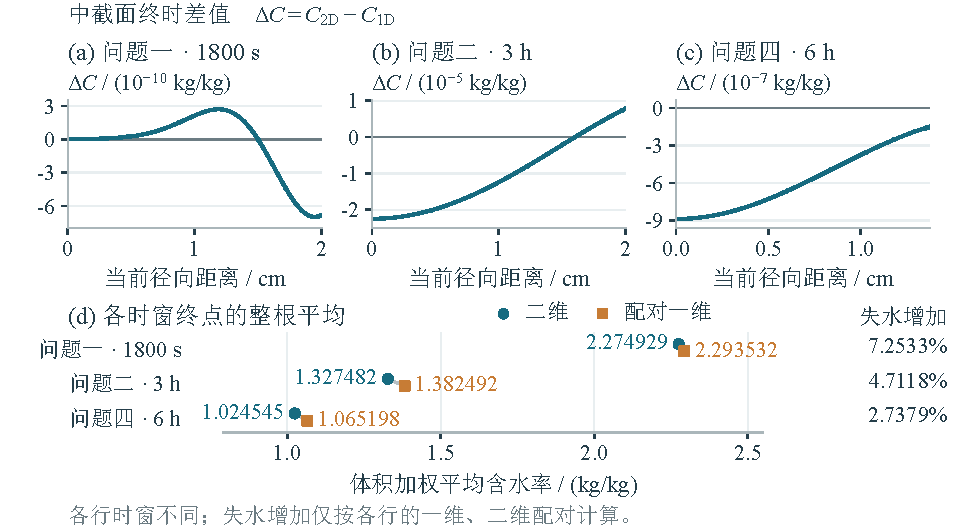
\includegraphics[width=.98\linewidth]{figures/legibility_validation/dimension_reduction.pdf}
\caption{已保存一维、二维配对场的降维证据：上排为问题一1800\unit{s}、问题二10800\unit{s}及问题四21600\unit{s}的中截面径向含水率差$\Delta C=C_{2D}-C_{1D}$；下排为各时窗终点的整根体积加权平均，圆点、方点分别表示二维和配对一维，终点失水增加与表\ref{tab:wholebody}一致。
问题一、二在已检时段中截面采样最大含水率差分别为$4.09\times10^{-9}$、$2.24706\times10^{-5}\unit{kg/kg}$。
上述时段最大差与上排终点差值的统计范围不同。
体积加权平均在空间均匀干密度假设下等于干质量加权平均。
数据取自同网格一维、二维配对保存场，文件索引与哈希见支撑材料图表来源清单；二维半柱坐标的$z=0$为中截面对称面。}
\label{fig:dimension-reduction}
\end{figure}
中截面差小与整根总量差可见并不矛盾。若用于全长平均、总失水或端部状态，应采用二维积分或明确忽略端面的近似，不能把中截面表格的精度扩展到全部工程指标。

上述中截面与整根积分对照用于评价降维近似，不能据此直接判定第四问的全域干燥终点。温度场与含水率相互耦合；即使$D$随温度增加，两个解之间的变系数通量散度也未必具有统一符号，因而不能将端面交换使干燥提前视为一般比较定理。

\subsection{后段环境的受控情景}
\label{sec:environment-scenarios}
由于式\eqref{eq:future}仅为4\unit{h}后的延拓，保持短时实测过程不变，从保存的4\unit{h}内部温湿场开展后段联立续算。每问设置原平台、温度$\pm1\unit K$和有效边界$b\pm0.005$五种情景；第四问始终使用同一观测$R(t)$。扰动幅度为人为选择的压力测试，没有作为测量不确定度或置信区间。表\ref{tab:environment}给出40阶配点的等号事件根，差值相对于同阶基线。
\begin{table}[htbp]
\centering\small
\caption{4\unit{h}后环境改变的条件根与时长差}\label{tab:environment}
\begin{tabular}{@{}lrrrr@{}}
\toprule 情景&问题三根/h&变化/h&问题四根/h&变化/h\\\midrule
原均值平台&57.473996&0&51.092003&0\\
$T_a-1\unit K$&59.341275&$+1.867279$&52.729346&$+1.637343$\\
$T_a+1\unit K$&55.688357&$-1.785639$&49.525343&$-1.566660$\\
$b-0.005$&57.382748&$-0.091249$&50.993818&$-0.098185$\\
$b+0.005$&57.584113&$+0.110117$&51.218753&$+0.126750$\\
\bottomrule
\end{tabular}
\end{table}
\begin{figure}[htbp]
\centering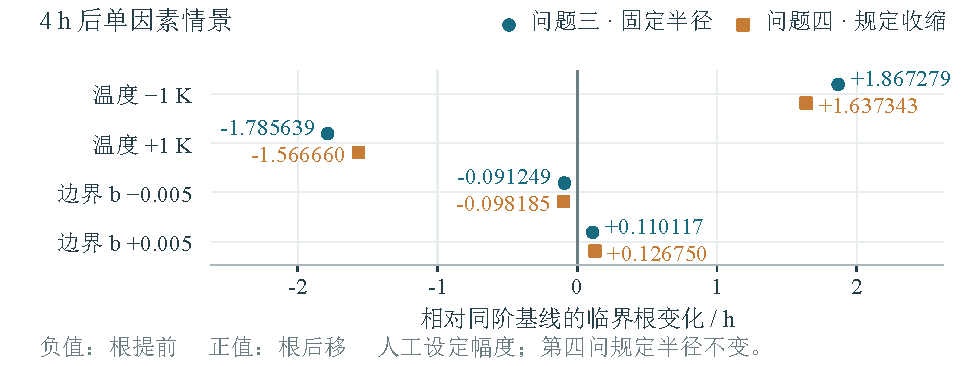
\includegraphics[width=.93\linewidth]{figures/legibility_validation/environment_sensitivity.pdf}
\caption{后段环境情景相对同阶基线的根变化；幅度为人工设定，第四问规定半径保持不变。圆点、方点分别表示问题三、四，共用零线；负值表示根提前，正值表示根后移。}\label{fig:environment}
\end{figure}
\FloatBarrier

对基线和降1\unit K情景进一步加密：问题三40阶到80阶、问题四40阶到60阶，单个根的最大变化分别约0.002951\unit{s}与0.000174\unit{s}，降温净效应的变化更小。因此小时级差不是此次降阶造成的；其他扰动没有逐一加密，表中六位小数仅便于追踪数值，不代表真实预测精度。

长期降温在既定模型内减小扩散温度因子，推迟阈值；提高$b$减小失水驱动力，也使根后移。由于两类扰动尺度不同，不能据图\ref{fig:environment}断定温度比所有湿度误差都重要。已有时间加权均值对照使问题三根变化约20.04\unit{s}，问题四改用PCHIP半径插值使根提前约12.61\unit{s}，二者也超过亚秒级一维经验数值预算。工程执行余量应建立在可用工况范围上，不能只依据四位小时的取整步长。

\section{模型评价、适用范围与推广}
\subsection{模型优点}
本文的优势体现在模型、数值实现与结果证据之间的对应关系，适用范围限于已声明的有效方程与工况。
\begin{enumerate}
\item \textbf{四问采用共同收支框架。}第\ref{sec:common-model}节统一热量、水分与材料运动的关系，各问再代入物性、几何和停止条件，便于区分变物性、终点判定与观测收缩的作用。
\item \textbf{圆环离散可核查总量收支。}第一问相邻控制体共享面通量，内部交换在求和时抵消，式\eqref{eq:q1-balance}将加权平均变化与表面交换对应，可用于检查离散总量一致性。
\item \textbf{原函数改写保持扩散通量。}式\eqref{eq:primitive}把可分离扩散率写为温度因子与原函数梯度的乘积，允许插值较平缓的原函数后反求含水率，保留题给非线性关系。
\item \textbf{终点判断兼顾内部极值与时间裕量。}式\eqref{eq:q3-extrema-candidates}--\eqref{eq:q3-reconstructed-max}检查径向重构的全部实驻点及端点，式\eqref{eq:event}区分等号临界根与严格执行时刻，避免用已舍入表值代替阈值判断。
\item \textbf{材料坐标避免重复计入收缩。}第\ref{sec:q4}节由组分守恒推导固定参考域方程，干基含水率无额外浓缩项；无交换纯收缩检验保持初态温湿与干、水质量，与所选材料运动一致。
\item \textbf{验证与输出来源分层可追溯。}第\ref{sec:q1}、\ref{sec:q2}节以独立算法和加密结果交叉核验，规定表值由对应未舍入数组生成；二维节点、配对估计与连续严格界分开报告，便于辨认结论由哪一级证据支持。
\end{enumerate}

\subsection{模型推广}
\label{sec:model-extension}
对具有同类有效物性与交换系数的圆柱形农产品，可将物性公式、环境记录和目标含水率作为替换接口，沿用控制体收支、离散组装与终点检测流程；迁移前须核对参数的单位、质量基准及适用温湿区间。本文未用其他物料作验证。

几何推广可从第\ref{sec:dimension-validation}节的一维径向与轴对称二维配对出发，在共同收支方程中替换散度算子、控制体权重及边界面。其他几何仍须重新处理对称条件、表面交换和网格检验，不能沿用本题的降维精度。对于以空间最大值限制工艺终点的其他状态量，若有可求极值的空间重构和明确的时间穿越方向，可移植“空间极值搜索、等号根定位、执行裕量复核”的事件流程，并按该变量重新设置阈值与误差预算。

对于已知外半径历程的物料，可用材料坐标组织输入，并按干物质守恒建立随动权重；内部运动仍需独立依据，仅有外半径不能唯一确定内部变形。取得后段工况记录后，第\ref{sec:environment-scenarios}节的单因素情景框架可用于比较允许工况范围内的终点变化，为工艺余量选择提供条件依据；本题人工扰动幅度不直接移作其他物料的余量。

\begingroup
\setlength{\parskip}{0pt}
\subsection{适用范围与主要限制}
\label{sec:limitations}
题表距离按中截面径向解释并作二维校核，并非题面指定的位置。

\textbf{气固边界与目标可达性。}材料$C$与空气$y_a$即使同写\unit{kg/kg}，分母也未必相同；湿度比、相对湿度与蒸气浓度须区分\cite{ashrae}。真实气膜候选边界为
\begin{equation}
j_s=k_g\{c_{v,s}(C_s,T_s)-c_{v,a}\},
\label{eq:physical-interface}
\end{equation}
其中$c_{v,s}$需材料水活度或解吸关系。仅当$c_{v,s}-c_{v,a}\approx K(C_s-b)$时，才能建立$\rhod h_m=k_gK$，不能直接交换系数数值。相关模型采用平衡干基含水率或气相/解吸关系\cite{dasilva2014,adrover2020}，未提供本药材标定值。须先核实目标环境下$C_{\mathrm{eq}}<0.15$；若$C_{\mathrm{eq}}\ge0.15$，从较高含水率开始的扩散干燥可能无法实现全域严格阈值，加密网格不能消除不可达性，未经标定的边界情景也不能称为实测。

\textbf{经验密度与材料质量的相容性。}若将题给$\rho=a+b_\rho C$同时解释为真实当前湿体密度，干基定义要求
\begin{equation}
\rhod(C)=\frac{a+b_\rho C}{1+C},\qquad
\frac{\dd\rhod}{\dd C}=\frac{b_\rho-a}{(1+C)^2}.
\end{equation}
这与前三问固定骨架的恒定干密度、第四问仿射收缩的空间均匀干密度不相容。本文仅将题给$\rho$用于有效容量，是建模处置而非题面规定。按第四问保存场强制采用真实湿密度解释，7\unit{h}和末态隐含干质量相对初值为0.71952、0.89029；保持$C,R$场不变，凑足总干质量需使长度由25\unit{cm}增至34.7454\unit{cm}与28.0807\unit{cm}。轴向收缩不能修复缺口，伸长凑平总量也未解决局部相容性；该反例不等于独立干质量账本数值泄漏，也不是可行伸长模型。

\textbf{相变能量与可报告的指标。}式\eqref{eq:heat}未显式计入相变能量，有限的$\rhoe c_p$不能在近等温持续失水时自动补充汽化功率。在“初始湿密度确定干质量、全部等效失水均蒸发”的附加条件下，取诊断常数$\lambda=2.45\unit{MJ/kg}$\cite{fao}，问题一1800\unit{s}的潜热需求约45.59\unit{kJ}，原轨迹对流输入约4.801\unit{kJ}，比例约9.50。问题四12\unit{h}表面近于环境温度、原轨迹净对流输入接近零，条件潜热通量$\lambda\rhod h_m(C_s-b)$仍约164.10\unit{W/m^2}。这些量级表明相变能量缺口尚未闭合，并非实际热量测量；重新联立相变会改变表面温度、热输入和扩散，不能固定原热输入倍乘干燥时间。现稿可报告有效模型的温湿分布、阈值事件和条件时长差，不能据此推断真实热量收支或执行保证。

\textbf{数值证据与工况的适用层级。}第三问57.4741\unit{h}的工程保守方向由二维终点节点场和配对根差支持，局部续算继承的前史误差仍需区分，不能将该时长解释为精确的二维最短时间；第四问51.0921\unit{h}为所设条件下的一维径向模型执行时长，已有粗网格二维核查在该时刻的最大含水率略高于阈值，有限圆柱全域达标尚待进一步验证，相关记录见支撑材料。两问均未取得连续二维严格误差界，也不能把条件时长作为实际工况保证。后段人为情景的幅度与用途见第\ref{sec:environment-scenarios}节，数值余量不覆盖环境、气固映射与物性假设的不确定性。
半径重建方案间的差异属于输入处理敏感性，不给出测量置信区间；复现规定的观测半径也不验证温湿预测，改变工况而沿用该历程时仅能报告条件响应。
\par\endgroup

\FloatBarrier
\Needspace{9\baselineskip}
\section*{AI工具使用声明}
\label{ai:declaration}
本参赛队在竞赛过程中使用了AI工具，主要用于求解代码编写、文献检索和语言润色，详细使用情况见支撑材料。

核心模型建立与论文初稿由参赛队完成。AI给出的求解代码和文献检索结果均经队员检查、修改和核验后采用；语言润色不改变模型、公式与数值结论。
\begin{thebibliography}{99}
\small
\setlength{\itemsep}{1pt}
\setlength{\parsep}{0pt}
\setlength{\parskip}{0pt}

\bibitem{dasilva2014}
da Silva W P, e Silva C M D P S, Gama F J A.
Estimation of thermo-physical properties of products with cylindrical shape
during drying: The coupling between mass and heat[J].
Journal of Food Engineering, 2014, 141: 65--73.
\href{https://doi.org/10.1016/j.jfoodeng.2014.05.010}{DOI:10.1016/j.jfoodeng.2014.05.010}.

\bibitem{adrover2020}
Adrover A, Venditti C, Brasiello A.
A Non-Isothermal Moving-Boundary Model for Continuous and Intermittent
Drying of Pears[J]. Foods, 2020, 9(11): 1577.
\href{https://doi.org/10.3390/foods9111577}{DOI:10.3390/foods9111577}.

\bibitem{wu2022}
吴孟秋, 雷登文, 朱广飞, 谢永康, 李星仪, 刘嫣红.
基于动网格的白萝卜热风干燥热质传递研究[J].
农业机械学报, 2022, 53(S2): 293--302.
\href{https://doi.org/10.6041/j.issn.1000-1298.2022.S2.034}{DOI:10.6041/j.issn.1000-1298.2022.S2.034}.

\bibitem{scipy}
SciPy developers.
scipy.integrate.solve\_ivp: SciPy v1.18.0 Manual[EB/OL]. [2026-09-12].
\url{https://docs.scipy.org/doc/scipy-1.18.0/reference/generated/scipy.integrate.solve_ivp.html}.

\bibitem{ashrae}
ASHRAE.
2021 ASHRAE Handbook---Fundamentals (SI Edition):
Chapter 1, Psychrometrics[M/OL]. 2021[2026-09-12].
\url{https://handbook.ashrae.org/Handbooks/F21/SI/F21_Ch01/F21_Ch01_si.aspx}.

\bibitem{fao}
Allen R G, Pereira L S, Raes D, Smith M.
Crop Evapotranspiration: Guidelines for Computing Crop Water Requirements[M/OL].
FAO Irrigation and Drainage Paper 56. Rome: FAO, 1998.
Chapter 3, Meteorological Data[2026-09-12].
\url{https://www.fao.org/4/X0490E/x0490e07.htm}.

\end{thebibliography}

\FloatBarrier
\par\clearpage\endgroup
\ifdefined\BodyOnly
\else
\clearpage
\appendix
\label{appendix:start}
\section{支撑材料与完整采用代码}
\label{sec:complete-code}
支撑包包含完整求解源码、题面附件、提交结果与数值复现入口。下列原求解代码保留；新增的完整复现控制、常规Excel导出、逐格核对及数值图生成代码一并列于本附录。代码附录不计入正文页数。

\codegroup{完整复现入口与验收范围}
在新的Python环境中安装支撑包的\texttt{requirements.txt}，运行\texttt{python -X utf8 reproduce.py --out ../reproduced --jobs 2}。程序仅以包内源码和题目附件重新计算四问主解、数值与二维对照、交换系数及后段环境情景，再核对论文表格、终点和提交结果。包内已有结果仅供比较，不作为求解初态。

输出目录包含新算的未舍入场、实际命令及退出码、独立工作簿读回、比较记录和数值核查图。第二问新生成的\texttt{result2.xlsx}包含完整全过程；压缩提交包中的同名小工作簿保存前三小时，全过程另以\texttt{NPZ}提供。新导出入口使用Python标准库与openpyxl，无需专有工作簿运行时。旧版导出代码保留以供追溯。

六张题设表按论文显示精度逐格比较；临界根和未舍入量使用记录在核验程序中的数值容差。复现结果不改变模型的条件性，也不将第四问一维执行值提升为有限圆柱连续全域的严格保证。运行方法及结果见支撑包的复现说明与验收记录。

\codegroup{原求解与诊断源码}
\sourcecode{匿名快照启动与冒烟检查}{support/launch.py}

\codegroup{第一问求解及交付}
\sourcecode{run\_all}{support/project/q1_complete_delivery/q1_delivery/run_all.py}

\sourcecode{q1\_solver}{support/project/q1_complete_delivery/q1_delivery/source/q1_solver.py}

\sourcecode{q1\_validate}{support/project/q1_complete_delivery/q1_delivery/source/q1_validate.py}

\sourcecode{q1\_refine}{support/project/q1_complete_delivery/q1_delivery/source/q1_refine.py}

\sourcecode{q1\_rounding\_audit}{support/project/q1_complete_delivery/q1_delivery/source/q1_rounding_audit.py}

\sourcecode{q1\_excel}{support/project/q1_complete_delivery/q1_delivery/source/q1_excel.py}

\sourcecode{q1\_report}{support/project/q1_complete_delivery/q1_delivery/source/q1_report.py}

\codegroup{第二问机制与参数情景}
\sourcecode{q2\_core}{support/project/q2_refinement_delivery/runtime/source/q2_core.py}

\sourcecode{q2\_spectral}{support/project/q2_refinement_delivery/runtime/source/q2_spectral.py}

\sourcecode{q2\_tests}{support/project/q2_refinement_delivery/runtime/source/q2_tests.py}

\sourcecode{q2\_core\_original}{support/project/q2_refinement_delivery/reused/q2_core_original.py}

\sourcecode{prepare\_reused}{support/project/q2_refinement_delivery/source/prepare_reused.py}

\sourcecode{q2\_mechanism}{support/project/q2_refinement_delivery/source/q2_mechanism.py}

\codegroup{第二三问全程统一轨迹}
\sourcecode{q3\_solver}{support/project/q4_complete_delivery/v1/q123_closeout/source/legacy_q3/q3_solver.py}

\sourcecode{q3\_reference}{support/project/q4_complete_delivery/v1/q123_closeout/source/legacy_q3/q3_reference.py}

\sourcecode{solve\_unified\_q23}{support/project/q4_complete_delivery/v1/q123_closeout/source/solve_unified_q23.py}

\sourcecode{audit\_unified\_q23}{support/project/q4_complete_delivery/v1/q123_closeout/source/audit_unified_q23.py}

\codegroup{第三问现行执行点与核验}
\sourcecode{q3\_solver}{support/project/q3_refinement_delivery/source/q3_solver.py}

\sourcecode{q3\_reference}{support/project/q3_refinement_delivery/source/q3_reference.py}

\sourcecode{q3\_refined\_reference}{support/project/q3_refinement_delivery/source/q3_refined_reference.py}

\sourcecode{future\_scenarios\_from\_checkpoint}{support/project/q3_refinement_delivery/source/future_scenarios_from_checkpoint.py}

\sourcecode{export\_workbook}{support/project/q3_refinement_delivery/source/export_workbook.py}

\sourcecode{validate\_xlsx}{support/project/q3_refinement_delivery/source/validate_xlsx.py}

\sourcecode{verify\_frozen}{support/project/q3_refinement_delivery/source/verify_frozen.py}

\codegroup{第四问及有限圆柱验证}
\sourcecode{q4\_common}{support/project/q4_complete_delivery/v1/source/q4_common.py}

\sourcecode{q4\_spectral}{support/project/q4_complete_delivery/v1/source/q4_spectral.py}

\sourcecode{run\_q4}{support/project/q4_complete_delivery/v1/source/run_q4.py}

\sourcecode{check\_numerics}{support/project/q4_complete_delivery/v1/source/check_numerics.py}

\sourcecode{finalize\_q4}{support/project/q4_complete_delivery/v1/source/finalize_q4.py}

\sourcecode{package\_workbooks}{support/project/q4_complete_delivery/v1/source/package_workbooks.py}

\sourcecode{export\_workbooks}{support/project/q4_complete_delivery/v1/source/export_workbooks.mjs}

\sourcecode{geometry\_solver\_executed}{support/project/q4_complete_delivery/v1/source/geometry_solver_executed.py}

\sourcecode{geometry\_solver}{support/project/q4_complete_delivery/v1/source/geometry_solver.py}

\sourcecode{geometry\_checks}{support/project/q4_complete_delivery/v1/source/geometry_checks.py}

\sourcecode{geometry\_analysis}{support/project/q4_complete_delivery/v1/source/geometry_analysis.py}

\sourcecode{geometry\_report}{support/project/q4_complete_delivery/v1/source/geometry_report.py}

\codegroup{本次整体复审}
\sourcecode{diagnose\_saved\_fields}{support/project/q1234_overall_review_delivery/v1/reviews/physics/diagnose_saved_fields.py}

\sourcecode{environment\_probe}{support/project/q1234_overall_review_delivery/v1/source/environment_probe.py}

\sourcecode{audit\_environment\_evidence}{support/project/q1234_overall_review_delivery/v1/reviews/environment_check/audit_environment_evidence.py}

\sourcecode{audit\_saved\_geometry\_scope}{support/project/q1234_overall_review_delivery/v1/reviews/geometry/audit_saved_geometry_scope.py}

\sourcecode{audit\_geometry\_endpoints}{support/project/q1234_overall_review_delivery/v1/reviews/geometry/audit_geometry_endpoints.py}

\codegroup{本稿图表后处理}
\sourcecode{build\_assets}{support/project/paper/q1234_draft_v1/build_assets.py}


\codegroup{新增完整复现与常规导出代码}
\sourcecode{reproduce}{reproduce.py}

\sourcecode{figures}{reproduction/figures.py}

\sourcecode{material\_motion}{reproduction/material_motion.py}

\sourcecode{portable\_workbooks}{reproduction/portable_workbooks.py}

\sourcecode{postprocess}{reproduction/postprocess.py}

\sourcecode{supplement}{reproduction/supplement.py}

\sourcecode{verify}{reproduction/verify.py}


\fi
\label{document:end}
\end{document}
